%class
	\documentclass{beamer}

%template
	\usetheme{HannoverSalman}
	\setbeamertemplate{navigation symbols}{}
	%\setbeamertemplate{footline}{\centering{\insertframenumber/\insertpresentationendpage}}
	%\setbeamertemplate{footline}{\hspace*{.5cm}\scriptsize{\hfill\insertframenumber\hspace*{.5cm}}} 


%packages
	\usepackage{amsmath, amssymb, graphicx,cancel}
	\usepackage[absolute,overlay]{textpos}
	\usepackage{subfigure}
	\usepackage{caption}\captionsetup{labelformat=empty,labelsep=none}
	\usepackage{geometry}
	\geometry{verbose}
	\usepackage{color}
	\usepackage{xmpmulti}
	\usepackage[3D]{movie15}
	\usepackage{hyperref}
%	\usepackage{bookmark}
	\usepackage[open,openlevel=4,atend]{bookmark}
	%\bookmarksetup{color=blue}
	\usepackage{multirow}
	\usepackage[style=numeric,defernumbers, authoryear]{biblatex}
	%\usepackage[square,sort]{natbib}
	%\usepackage{fancyhdr}%\pagestyle{fancy} 

	
	\hypersetup{bookmarksdepth = 4}


%citations files
	\bibliography{MyCitations}

%logoCSIPCPL
    \setlength{\TPHorizModule}{1mm}
    \setlength{\TPVertModule}{1mm}
    \newcommand{\logoCSIPCPL}
    {
    	\begin{textblock}{1}(100,2) %(100,85)  for bottom
    		
\includegraphics[width=1.5cm]{figs/logo_CSIP}
    	\end{textblock}
    	
	\begin{textblock}{1}(117,1) %(117,85)  for bottom
    		
\includegraphics[width=1.0cm]{figs/logo_CPL}
    	\end{textblock} 
    }

%logo evolution
    \newcommand{\logoEvolution}
    {    	
	\begin{textblock}{1}(110,1) %(117,85)  for bottom
    		\includegraphics[width=0.65in]{figs/logo_evolution.pdf}
    	\end{textblock} 
    }

%logo Qualcomm
    \newcommand{\logoQualcomm}
    {
    	\begin{textblock}{1}(110,2) %(100,85)  for bottom
    		\includegraphics[width=1.5cm]{figs/logo_qualcomm.jpg}
    	\end{textblock}
    }
%logo Qualcomm (long)
    \newcommand{\logoQualcommllong}
    {
    	\begin{textblock}{1}(0,0) 
    		\includegraphics[width=1.25in]{figs/logo_qualcomm_long.jpg}
    	\end{textblock}
    }

%logo Tech Tower
    \newcommand{\logoTechTower}
    {
    	\begin{textblock}{1}(0,0) 
    		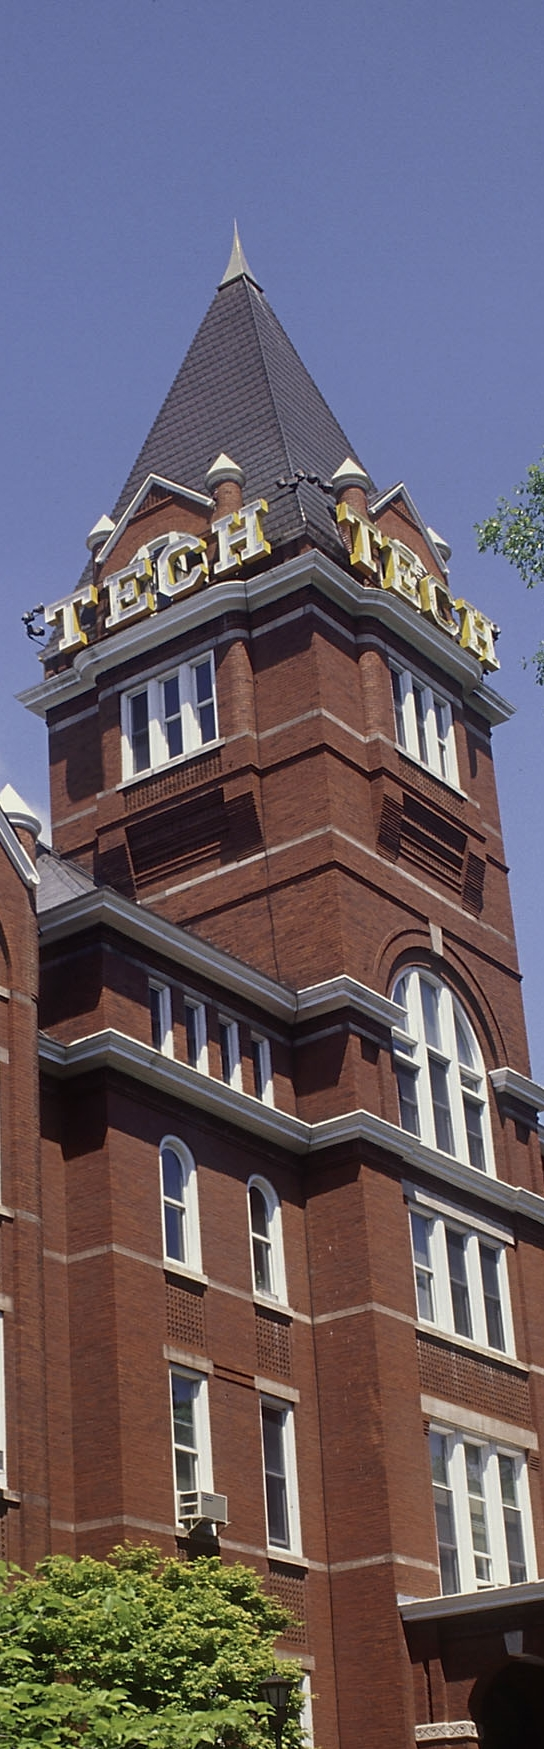
\includegraphics[width=1.25in]{figs/logo_TechTower.jpg}
    	\end{textblock}
    }

%logo tree
    \newcommand{\logoTree}
    {
    	\begin{textblock}{1}(0,0) 
    		\includegraphics[width=1.25in]{figs/logo_tree.jpg}
    	\end{textblock}
    }
%page numbers
    \newcommand{\mypagenum}
    {
    	\begin{textblock}{1}(1,94) 
		{\tiny \color[rgb]{0.2,0.2,1}\insertframenumber} %\insertframenumber,\insertpresentationendpage, \inserttotalframenumber
    	\end{textblock}
    }
%my footnote citation
	\newcommand{\myFootnoteCitation}[2]
	{
		\footnote{\tiny \citeauthor{#1}, \emph{#2}, \citeyear{#1}.}  %\citeauthor{#1}, \citetitle{#1}, #2 \citeyear{#1}.
	}
%my refer to citation
	\newcommand{\mycite}[1]
	{
		\emph{\citeauthor{#1} (\citeyear{#1})}
	}
%my footnote website citation
	\newcommand{\myFootnoteWebsiteCitation}[1]
	{
		\footnote{\tiny \citeauthor{#1}}
	}

\let\thefootnote\relax\footnotetext{Footnotetext without footnote mark}


%section underline
%\newcommand{\tmpsection}[1]{}
%\let\tmpsection=\section
%\renewcommand{\section}[1]{\tmpsection{\underline{#1}}}



%commands
	\newcommand{\likelihood}{p(Z_k| x_k) }						%likelihood
	\newcommand{\prior}{p(x_k)  } 								%prior
	\newcommand{\posterior} {p(x_k| Z_k)}						%posterior
	\newcommand{\prediction} {p(x_k| Z_{k-1})}					%prediction
	\newcommand{\update} {p(x_k|Z_k)}							%update
	\newcommand{\observations} {p(Z_k)}						%observations
	\newcommand{\prevobservations} {p(Z_{k-1})}				%previous observations
	\newcommand{\dxpk} {dx_{k-1}}							%dx_{k-1}
	\newcommand{\ChapKolm}{\int{p(x_k| x_{k-1})p(x_{k-1}|Z_{k-1})} \dxpk} %Chapman Kolmogorov

	%algorithm specific: JPDAF
	\newcommand{\likelihoodJPDAF}{p(Z_k| \chi, m, Z_{k-1}) }		%1. likelihood
	\newcommand{\priorJPDAF}{p(\chi|m, Z^{k-1}} 				%2. prior	
	\newcommand{\observationsJPDAF} {p(Z_k}					%3. observations
	\newcommand{\posteriorJPDAF} {p(\chi| Z_k)}					%4. posterior

%environments
	\newenvironment{changemargin}[2]
	{
	  	\begin{list}{}
		{
			\setlength{\topsep}{0pt}%
			\setlength{\leftmargin}{#1}%
			\setlength{\rightmargin}{#2}%
			\setlength{\listparindent}{\parindent}%
			\setlength{\itemindent}{\parindent}%
			\setlength{\parsep}{\parskip}%
		}
	  	\item[]
		}
		{\end{list}
	}
%figures

%colors
\definecolor{darkgreen}{rgb}{0,0.5,0}

%personal details
	\author{Salman Aslam}
	\institute{Advisor, Dr Christopher Barnes (ECE)\\Co-advisor, Dr Aaron Bobick (CoC)\\Georgia Institute of Technology}
	\date{}

\begin{document}
%####################################################################################################
\title{Multi-target Tracking \\ Using \\Residual Vector Quantization}
%####################################################################################################
\begin{frame}[plain]\logoCSIPCPL\logoTechTower
	\titlepage
\end{frame}

\begin{frame}
\frametitle{Outline}
\logoCSIPCPL\logoTechTower
	\setcounter{tocdepth}{2}	
	\tableofcontents
\end{frame}

%####################################################################################################
\section{I. Tracking: introduction}
%####################################################################################################
\begin{frame}
\frametitle{Tracking}
\framesubtitle{definition}
\logoCSIPCPL\mypagenum
	Estimate and maintain {\color{red}target state} over {\color{red}time}
	\begin{figure}
		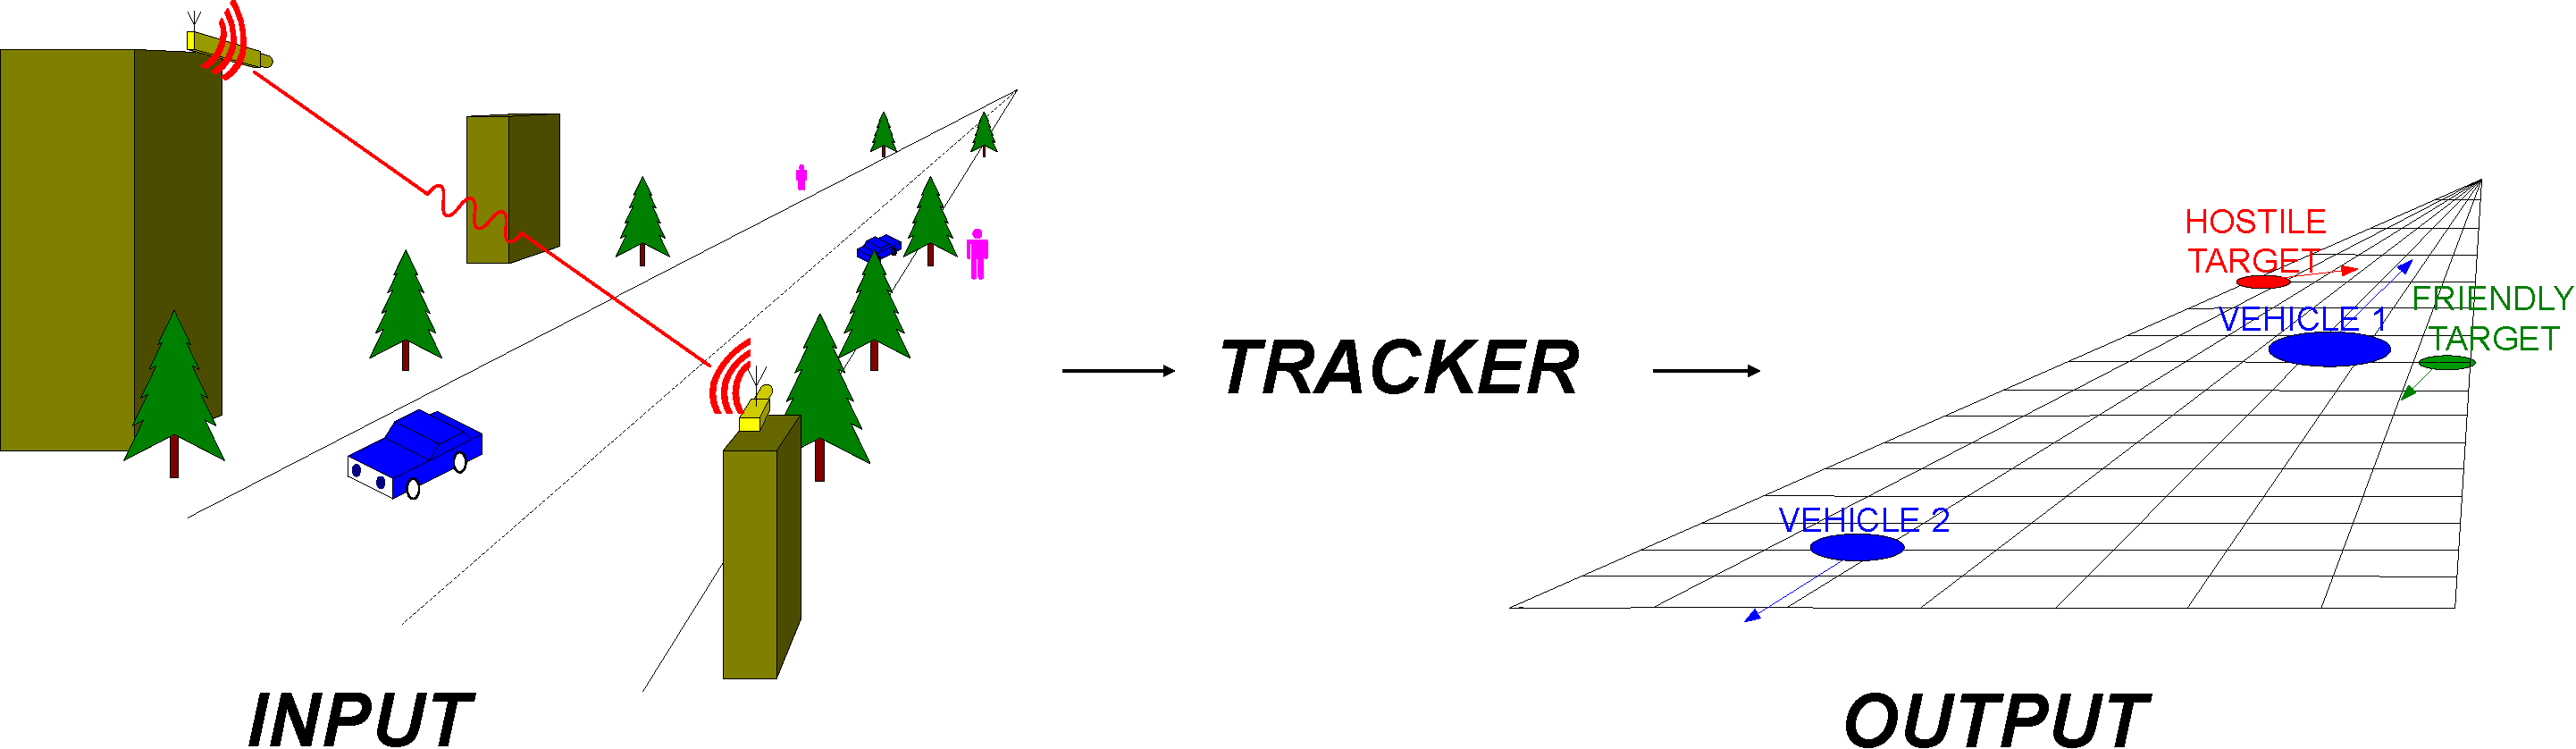
\includegraphics[width=1.0\textwidth]{figs/TRK_overviewDiagram.pdf}
	\end{figure}
\end{frame}


\begin{frame}[plain]
\frametitle{Tracking}
\framesubtitle{overview\tiny{\footnote {Yilmaz et.al., 2006}}}
\logoCSIPCPL\mypagenum
	\begin{changemargin}{-1.3in}{0in}
		\begin{figure}
			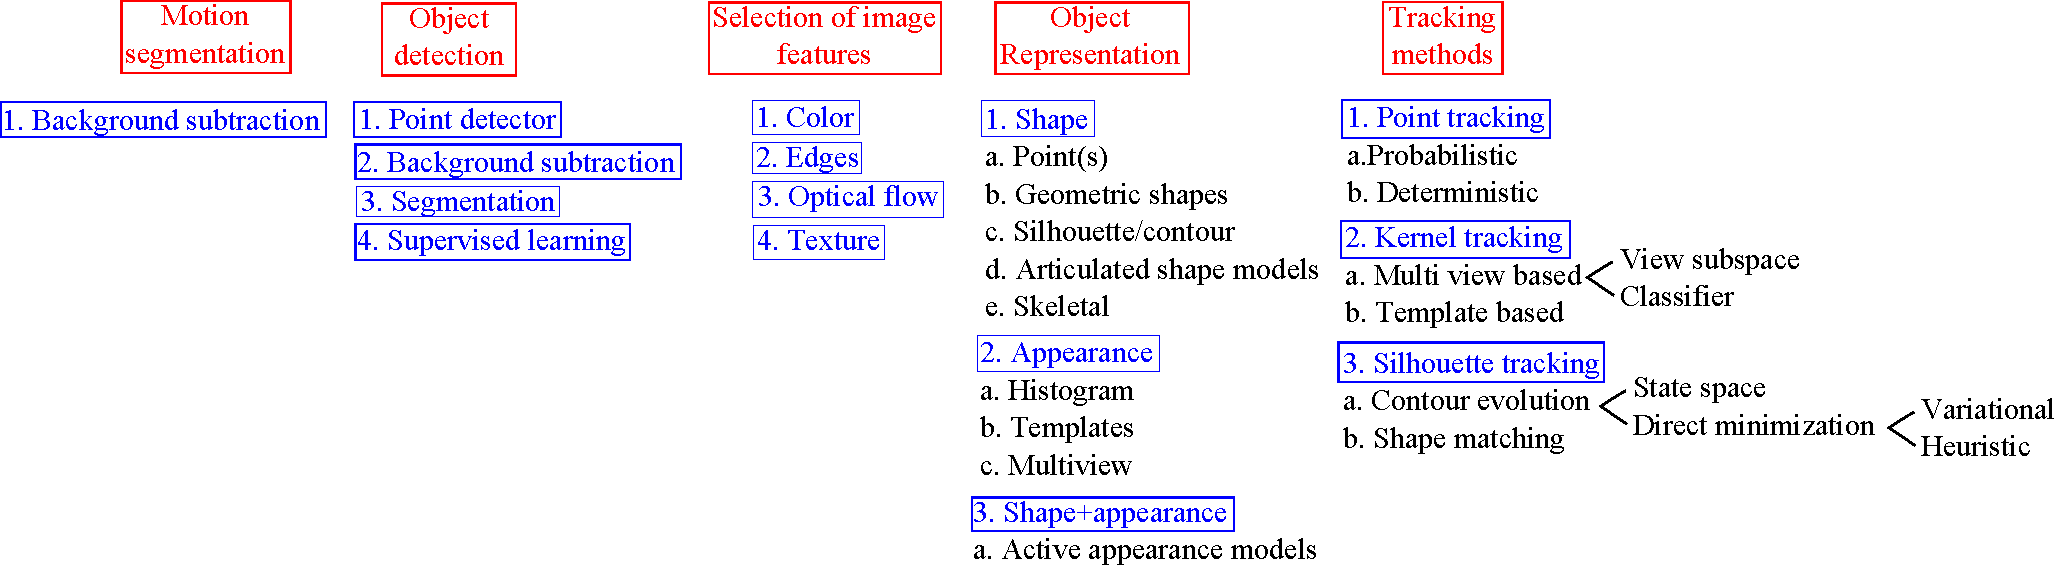
\includegraphics[width=1.3\textwidth]{figs/TRK_overview.pdf}
		\end{figure}	
	\end{changemargin}
	\begin{block}{Tracking methods}
		\begin{itemize}
			\item Point
			\item Region
			\item Contour
		\end{itemize}
	\end{block}
\end{frame}



\begin{frame}
\frametitle{Tracking}
\framesubtitle{big picture}
\logoCSIPCPL\mypagenum
	\begin{figure}
		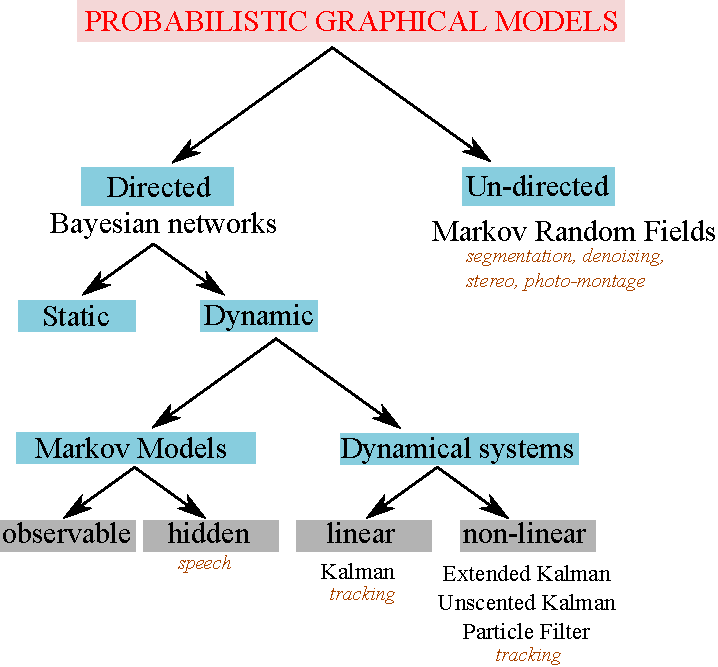
\includegraphics[width=0.9\textwidth]{figs/PRML_PGM_overview.pdf}
	\end{figure}
\end{frame}





\begin{frame}
\frametitle{Tracking}
\framesubtitle{relationship with HMM}
\logoCSIPCPL\mypagenum
	\begin{figure}
		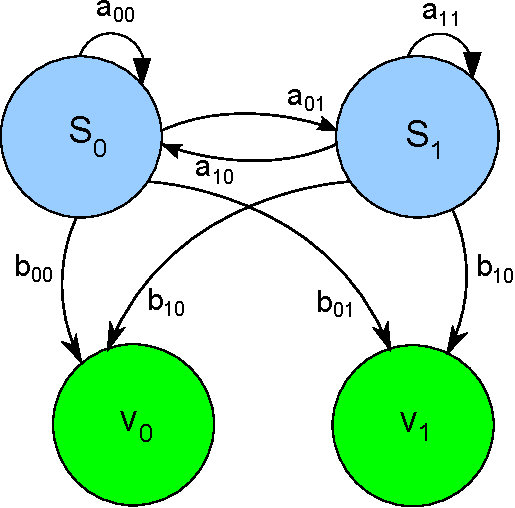
\includegraphics[height=0.3\textheight]{figs/HMM_flowDiagram.pdf}
	\end{figure}
	\begin{figure}
		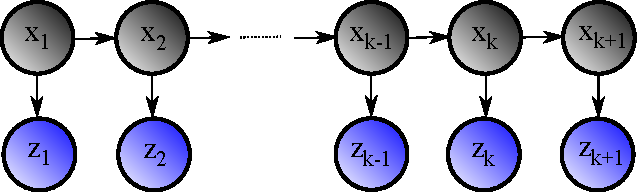
\includegraphics[width=1.0\textwidth]{figs/HMM_flowDiagram2.pdf}
	\end{figure}
\end{frame}



\begin{frame}
\frametitle{Tracking}
\framesubtitle{update}
\logoCSIPCPL\mypagenum
	\begin{figure}
		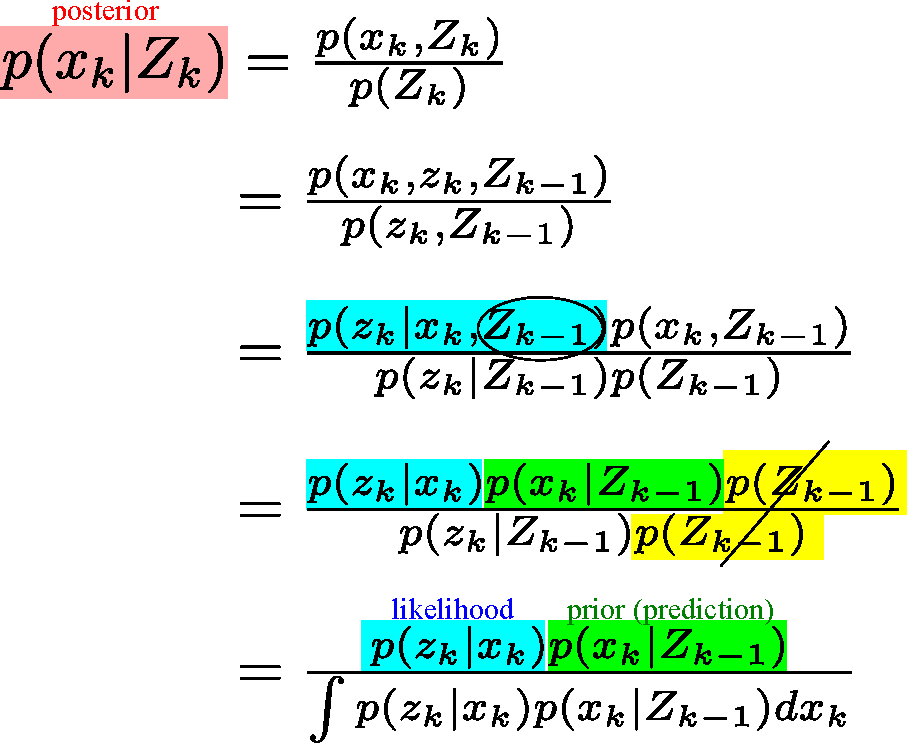
\includegraphics[width=1.0\textwidth]{figs/TRK_EQN_update.pdf}
	\end{figure}
\end{frame}



\begin{frame}
\frametitle{Tracking}
\framesubtitle{prediction}
\logoCSIPCPL\mypagenum
	Chapman Kolmogorov equation
	\begin{figure}
		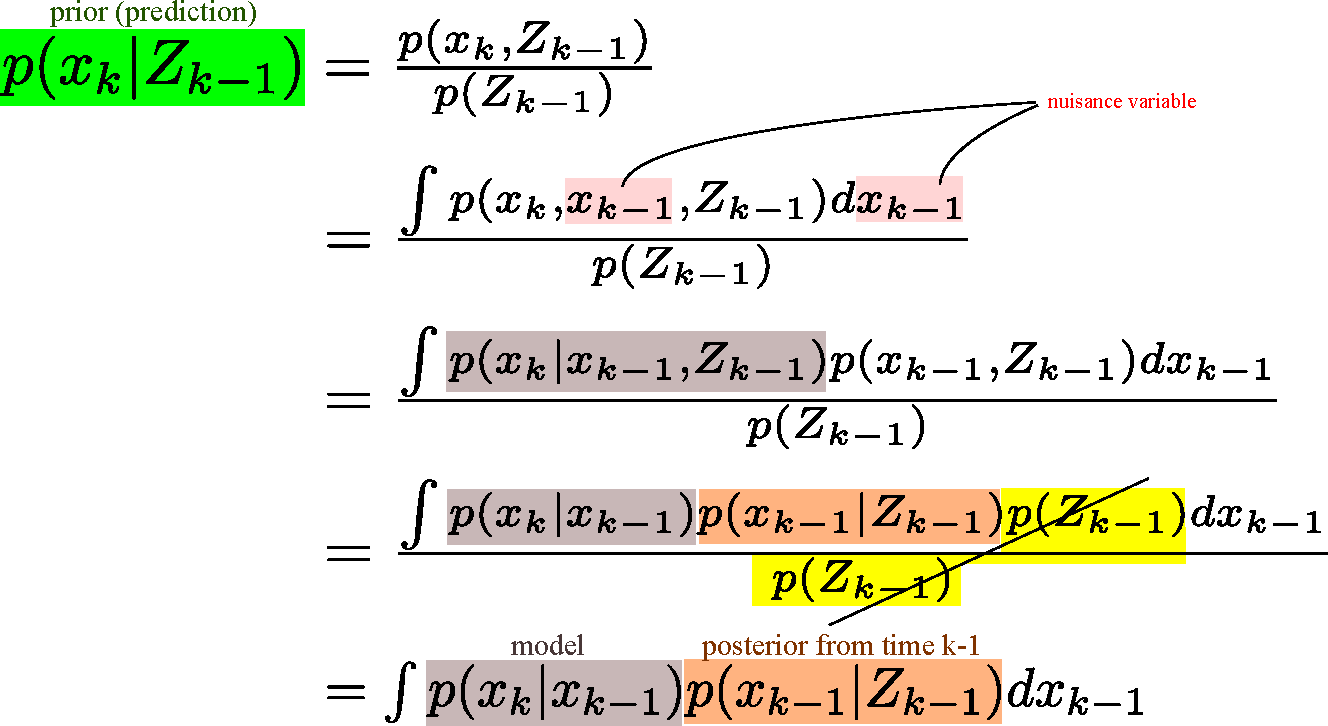
\includegraphics[width=1.0\textwidth]{figs/TRK_EQN_prediction.pdf}
	\end{figure}
\end{frame}


%#######################################################################
\section{II. Tracking: radar (points)}
%#######################################################################


%===================================================
\subsection{\ \ \ \ clutter-free}
%===================================================
%------------------------------------------------------------
\subsubsection{\ \ \ \ \ \ \ \ Kalman filter }
%------------------------------------------------------------


\begin{frame}
\frametitle{Kalman Filter}
\framesubtitle{block diagram}
\logoCSIPCPL\mypagenum
	\begin{figure}
		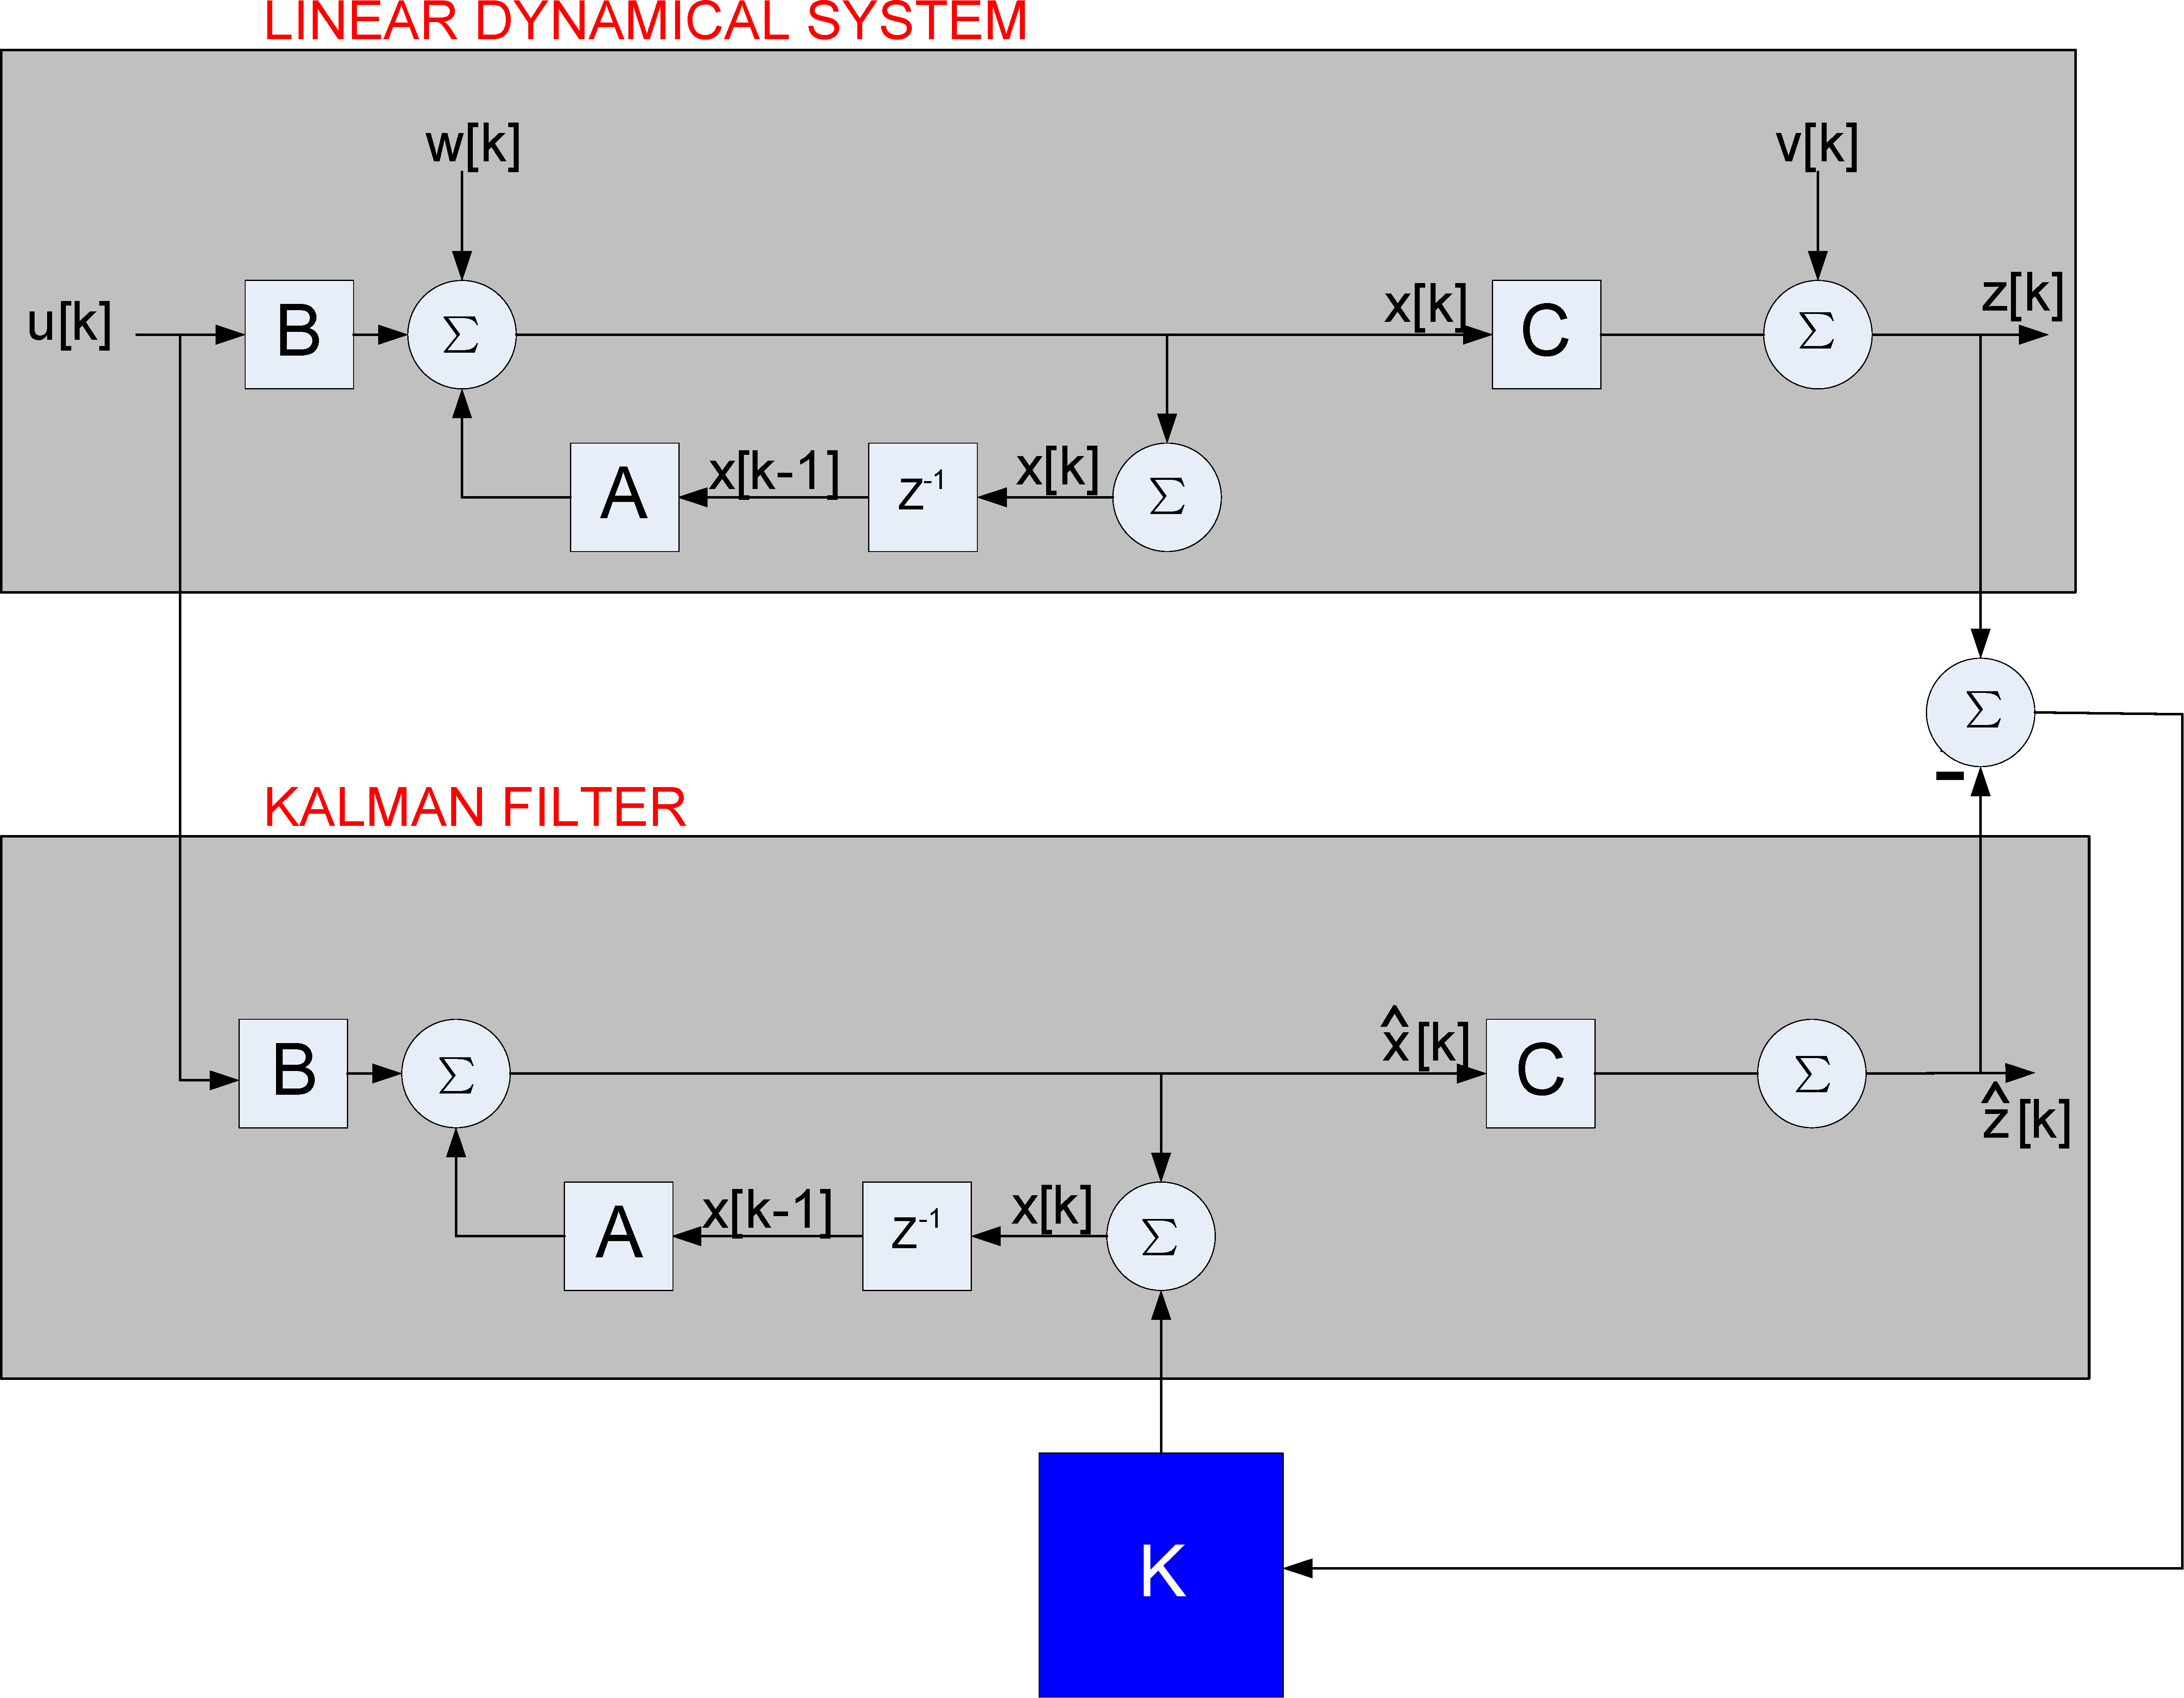
\includegraphics[width=1.0\textwidth]{figs/TRK_KalmanFilter_blockDiagram.pdf}
	\end{figure}
\end{frame}



%\begin{frame}
%\frametitle{Kalman Filter}
%\framesubtitle{overview}
%\logoCSIPCPL\mypagenum
%	\begin{itemize}
%		\item {\color{red}Prior}
%			\begin{itemize}
%				\item Past information through time $k-1$
%				\item summarized approximately by a sufficient statistic in the form of a Gaussian posterior
%			\end{itemize}
%		\begin{equation*}
%			p(x_{k-1|k-1}|Z_{k-1})=\mathcal{N}  (\hat{x}_{k-1|k-1}, P_{k-1|k-1})
%		\end{equation*}
%		\item {\color{red}Prediction}
%			\begin{itemize}  
%				\item The state prediction is distributed as,
%				\begin{equation*}
%					p(x_{k|k-1}|Z_{k-1})=\mathcal{N}  (\hat{x}_{k|k-1}, P_{k|k-1})
%				\end{equation*}
%				\item The observation prediction is distributed as,
%				\begin{equation*}
%					p(z_{k|k-1})=\mathcal{N}  (\hat{z}_{k|k-1}, S_k)
%				\end{equation*}
%			\end{itemize}
%		\item {\color{red}Update}
%			\begin{itemize} 
%				\item innovation
%				\item Kalman gain
%				\item aposteriori state estimate and aposteriori covariance estimate
%			\end{itemize}
%	\end{itemize}
%\end{frame}



\begin{frame}
\frametitle{Kalman Filter}
\framesubtitle{equations}
\logoCSIPCPL\mypagenum
	\begin{figure}
		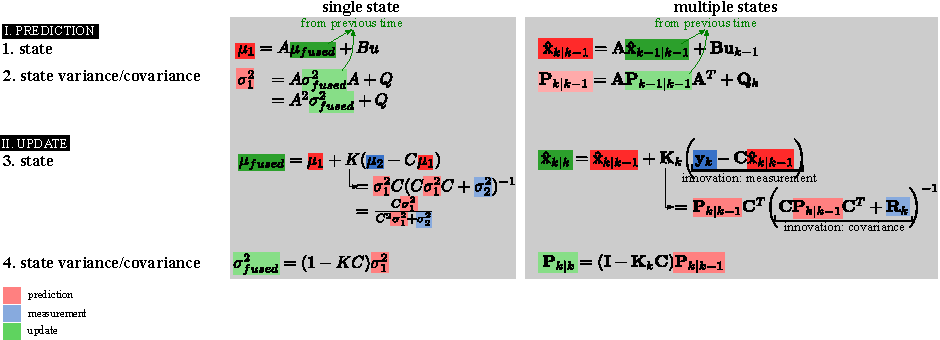
\includegraphics[width=1.0\textwidth]{figs/TRK_KalmanFilter_equations.pdf}
	\end{figure}
\end{frame}

%===================================================
\subsection{\ \ \ \ clutter}
%===================================================

%\begin{frame}\frametitle{Theory}\logoCSIPCPL\mypagenum
%	\begin{figure}
%		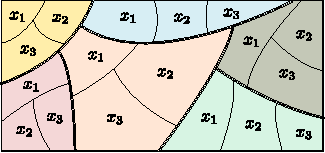
\includegraphics[width=0.7\textwidth]{figs/TRK_PDAF_probability_space.pdf}
%	\end{figure}
%\end{frame}

\begin{frame}[plain]
\frametitle{Tracking in clutter}
\frametitle{MMSE, MMSE-MAP, MMSE-ML}
\logoCSIPCPL\mypagenum
	\begin{changemargin}{-1.3in}{0in}
		\begin{figure}
			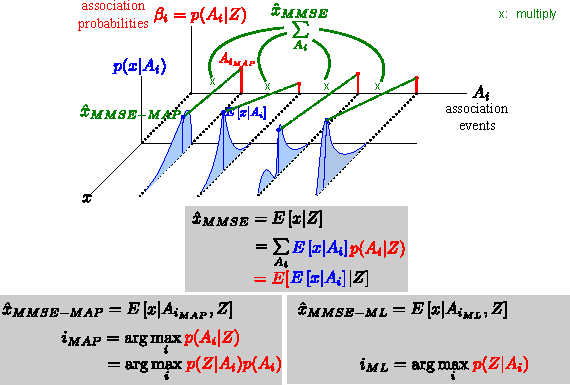
\includegraphics[width=1.3\textwidth]{figs/TRK_clutter_all.pdf}
		\end{figure}
	\end{changemargin}
\end{frame}



\begin{frame}
\frametitle{Tracking in clutter}
\framesubtitle{MMSE}
\logoCSIPCPL\mypagenum
	\begin{figure}
		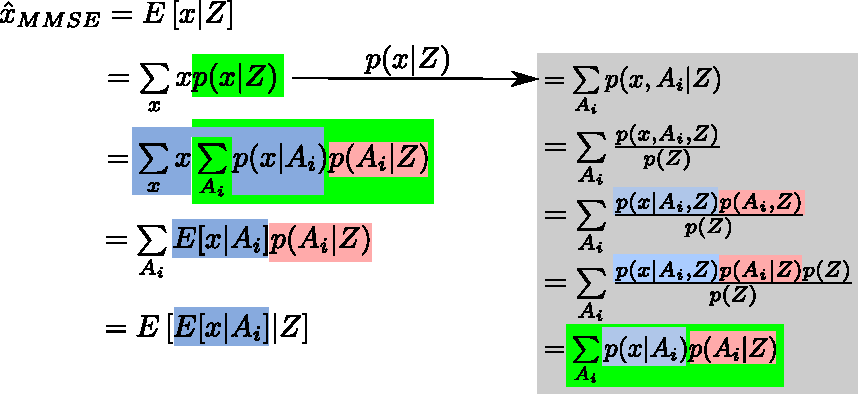
\includegraphics[width=1.0\textwidth]{figs/TRK_clutter_MMSE.pdf}
	\end{figure}
\end{frame}






%------------------------------------------------------------
\subsubsection{\ \ \ \ \ \ \ \ PDAF }
%------------------------------------------------------------
%\begin{frame}
%\frametitle{PDAF}
%\framesubtitle{Introduction}
%\logoCSIPCPL\mypagenum
%	{\color{red} Probabilistic Data Association Filter}
%	\begin{itemize}
%		\item Computationally efficient 
%		\item Data association
%		\item Single targets in clutter, high false alarm rate
%		\item Extension of Kalman filter
%		\begin{itemize}
%			\item Primary difference: computation of innovations
%			\item Calculates association probabilities to the target for each validated measurement
%		\end{itemize}
%	\end{itemize}
%\end{frame}



%\begin{frame}\frametitle{Other solutions}\logoCSIPCPL\mypagenum
%	\begin{itemize}
%		\item Standard filter: pick one of them, e.g. nearest neighbor (possibly incorrect)
%		\item Track split: one track for every possible measurement (computationally expensive)
%	\end{itemize}
%\end{frame}




%\begin{frame}
%\frametitle{PDAF}
%\framesubtitle{assumptions}
%\logoCSIPCPL\mypagenum
%	\begin{enumerate}
%		\item  {\color{red}{Number of targets}}
%		\begin{itemize}
%			\item Single target tracking
%		\end{itemize}
%		\item {\color{red}{False alarms}}
%		\begin{itemize} 
%			\item At most, one of the validated measurements can be target originated	
%			\item Remaining measurements
%			\begin{itemize}
%				\item incorrect, i.e., false alarms
%				\item i.i.d
%				\item parametric form: Poisson distribution with known spatial density $\lambda$
%				\item non-parametric form: uniform spatial distribution
%			\end{itemize}
%		\end{itemize}
%	\end{enumerate}
%\end{frame}
	



%\begin{frame}
%\frametitle{PDAF}
%\framesubtitle{assumptions (cont.)}
%\logoCSIPCPL\mypagenum
%	\begin{enumerate}\setcounter{enumi}{2}
%		\item {\color{red}{Target detection}}
%		\begin{itemize} 
%			\item Known probability, $P_D$
%		\end{itemize}
%		%\item Innovation of correct return normally distributed
%		\item {\color{red}{Prior}}
%		\begin{itemize} 
%			\item Density of the state conditioned on the past observations is a Gaussian distribution,		
%		\end{itemize}
%		\begin{equation*}
%			p(\mathbf{x}_{k-1}|Z^{k-1}) = \mathcal{N}  (  \hat{\mathbf{x}}_{k-1|k-1}, \mathbf{P}_{k-1|k-1})
%		\end{equation*}
%	\end{enumerate}
%\end{frame}



\begin{frame}[plain]
\frametitle{PDAF}
\framesubtitle{flow diagram \tiny{\footnote{Bar-shalom, 2009}}}
\logoCSIPCPL\mypagenum
	\begin{changemargin}{-1.3in}{0in}
		\begin{figure}
			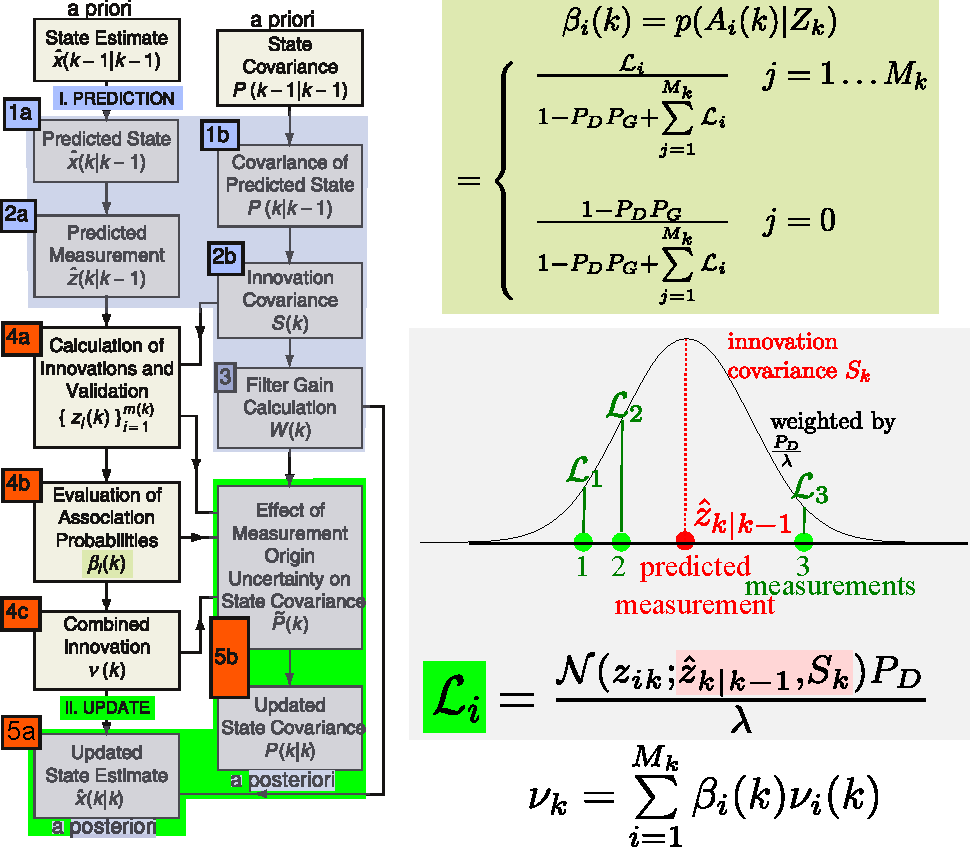
\includegraphics[height=0.8\textheight]{figs/TRK_PDAF_flowDiagram.pdf}
		\end{figure}	
	\end{changemargin}
\end{frame}





%\begin{frame}
%\frametitle{PDAF}
%\framesubtitle{innovations, step 1}
%\logoCSIPCPL\mypagenum
%	{\color{red}Measurement validation}
%	\begin{itemize} 
%		\item only measurements inside a validation gate are accepted. 
%		\item $P_G$: If the true measurement is detected,  $P_G$ is the probability that it is in the gate
%	\end{itemize}
%\end{frame}
%
%
%
%
%
%\begin{frame}
%\frametitle{PDAF}
%\framesubtitle{innovations, step 2}
%\logoCSIPCPL\mypagenum
%	\begin{itemize}
%		\item {\color{red} Association events, $A_i$}
%		\begin{itemize}
%			\item mutually exclusive and exhaustive
%			\item Example of three measurements
%			\begin{itemize}
%				\item $z_1$ originated from target, $z_2$ and $z_3$ are spurious
%				\item $z_2$ originated from target, $z_1$ and $z_3$ are spurious
%				\item $z_3$ originated from target, $z_1$ and $z_2$ are spurious
%				\item All are spurious
%			\end{itemize}
%		\end{itemize}
%		\item {\color{red} Association probabilities, $\beta_i$}
%		\begin{itemize}
%			\item $\beta_i$ the aposterior probability that the $i$-th return originated from the object in track
%			\item$\beta_0$ is the probability that none of the measurements are correct
%		\end{itemize}
%	\end{itemize}
%\end{frame}
%
%
%
%
%\begin{frame}
%\frametitle{PDAF}
%\framesubtitle{innovations, step 2 (cont.)}
%\logoCSIPCPL\mypagenum
%	Computing the association probabilities, $\beta_{ik}$,
%	\begin{align*}
%		\beta_{ik} &\triangleq p(A_{ik}|Z_k)\\
%				&=	\left\{ 
%						\begin{array}{cc}
%							\frac{\mathcal{L}_i}{1-P_DP_G + \sum\limits_{j=1}^{j=M_k} \mathcal{L}_i}  & j=1 \ldots M_k\\ \\
%							\frac{1-P_DP_G}{1-P_DP_G + \sum\limits_{j=1}^{j=M_k} \mathcal{L}_i} & j=0
%						\end{array} 
%					\right. \\
%		\mathcal{L}_i&= \frac{\mathcal{N}  (z_{ik};  \hat{z}_{k|k-1}, S_k)P_D}{\lambda}
%	\end{align*}
%\end{frame}
%
%
%
%
%\begin{frame}
%\frametitle{PDAF}
%\framesubtitle{innovations, step 2 (cont.)}
%\logoCSIPCPL\mypagenum	
%	\begin{align*}
%		\mathcal{L}_i&= \frac{\mathcal{N}  (z_{ik};  \hat{z}_{k|k-1}, S_k)P_D}{\lambda}
%	\end{align*}
%	\begin{itemize}
%		\item Likelihood $L_i$ is centered around the predicted observation
%		\begin{itemize}
%			\item Far away clutter has exponentially lower weight
%		\end{itemize}
%	\end{itemize}
%\end{frame}
%
%
%
%
%\begin{frame}
%\frametitle{PDAF}
%\framesubtitle{innovations, step 3}
%\logoCSIPCPL\mypagenum
%	{\color{red} Innovations, $\nu_{ik}$}
%	\begin{itemize}
%		\item $\mathbf{\nu}_{ik}$  for each measurement $\mathbf{z}_{ik}$ are computed using the conditional mean of the observations $\hat{\mathbf{z}}(k|k-1)$:
%		\begin{equation*}
%			\nu_{ik}  \triangleq \mathbf{z}_{ik} - \hat{\mathbf{z}}(k|k-1) 
%		\end{equation*}
%	\end{itemize}
%\end{frame}
%
%
%
%\begin{frame}
%\frametitle{PDAF}
%\framesubtitle{innovations, step 4}
%\logoCSIPCPL\mypagenum
%	{\color{red} Combined innovation, $y_k$}
%	\begin{itemize}
%		\item $\mathbf{\nu}_{ik}$ and $\beta_{ik}$ for each target are combined to form a combined innovation:  
%		\begin{equation*}
%			y_k  \triangleq \sum_{i=1}^{M_k} \beta_{ik}\nu_{ik}
%		\end{equation*}
%	\item If there is only one measurement, i.e., $M_k=1$, PDAF becomes equivalent to the Kalman Filter
%	\end{itemize}
%\end{frame}
%
%
%
%
%\begin{frame}
%\frametitle{PDAF}
%\framesubtitle{covariance update}
%\logoCSIPCPL\mypagenum
%	\begin{align*}
%		\mathbf{P}_{k|k-1} =
%		&\beta_{0k}\mathbf{P}_{k|k-1} +\\
%		&\left[1-\beta_{0k}\right]\left[\mathbf{P}_{k|k-1}-\mathbf{K}_k\mathbf{S}_k\mathbf{K}_k'\right] +\\
%		&\mathbf{K}_k\left[\sum\limits_{i=1}^{m_k}\beta_{ik}y_{ik}y_{ik}'-y_{k}y_{k}'\right]\mathbf{K}_k' 
%	\end{align*}
%\end{frame}
%
%
%
%
%\begin{frame}
%\frametitle{PDAF}
%\framesubtitle{limitations}
%\logoCSIPCPL\mypagenum
%	\begin{itemize}
%		\item The PDAF algorithm makes an assumption that a single target is being tracked.  
%		\item Additional targets handled with multiple copies of the filter.  
%		\item However, in such cases, measurements from interfering targets do not behave like a Poisson process.  
%		\item Solution: JPDAF
%	\end{itemize}
%\end{frame}



\begin{frame}
\frametitle{PDAF}
\framesubtitle{usage}
\logoCSIPCPL\mypagenum
	PDAF + multiple model Kalman Filters \tiny{\footnote{Bar-Shalom et al., 2009}}:
	\begin{figure}
		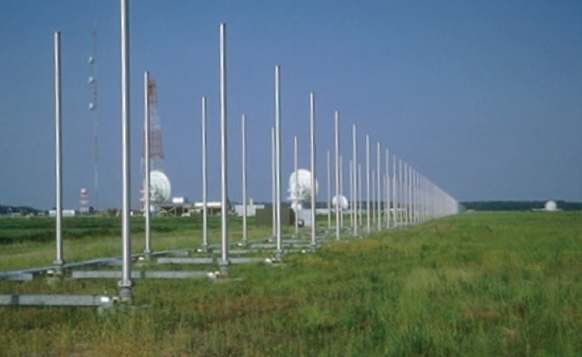
\includegraphics[width=0.8\textwidth]{figs/TRK_PDAF_example_US_Navy_ROTHR.jpg}
		\caption {US Navy ROHR (Relocatable Over the Horizon Radar) for long-range surveillance for drug interdiction against aircraft and ships}
	\end{figure}
\end{frame}

%------------------------------------------------------------
\subsubsection{\ \ \ \ \ \ \ \ JPDAF }
%------------------------------------------------------------
%\begin{frame}
%\frametitle{JPDAF}
%\framesubtitle{Introduction}
%\logoCSIPCPL\mypagenum
%	{\color{red} Joint Probabilistic Data Association Filter}
%	\begin{itemize}
%		\item Extension of PDAF to multi-target tracking	
%			\begin{itemize}
%				\item Only difference: computation of association probabilities, $\beta_{ik}$
%			\end{itemize}
%		\item Handles multiple targets by considering all measurements for all targets.  
%		\item Probability density of each candidate measurement
%			\begin{itemize}
%				\item Based on all close-by targets
%			\end{itemize}
%	\end{itemize}
%\end{frame}




\begin{frame}
\frametitle{JPDAF}
\framesubtitle{association probabilities}
\logoCSIPCPL\mypagenum 	
	\begin{figure}
		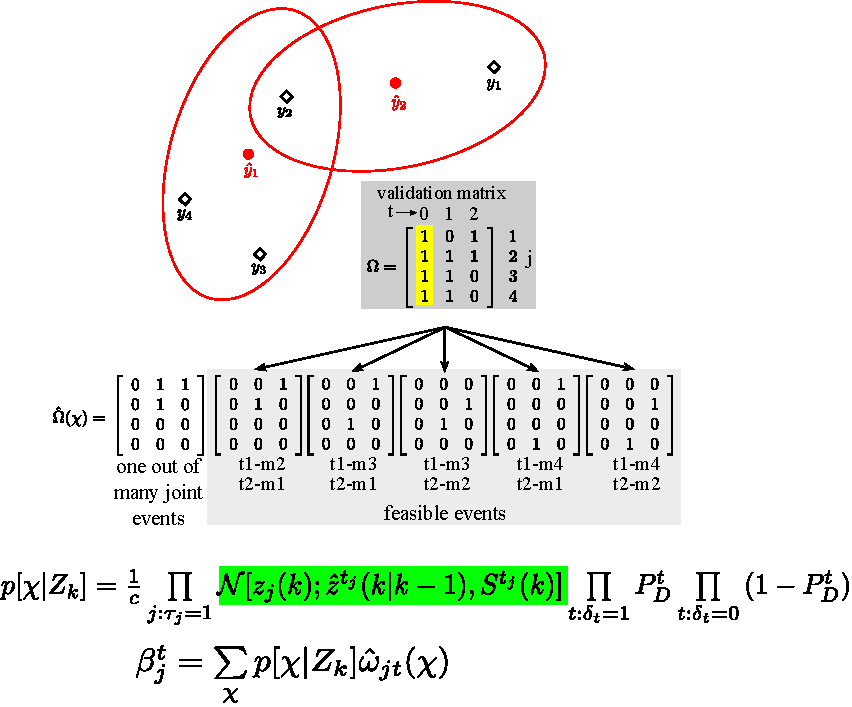
\includegraphics[height=0.80\textheight]{figs/TRK_JPDAF_twoTargetScenario.pdf}
	\end{figure}	
\end{frame}

%\begin{frame}\frametitle{JPDAF}\logoCSIPCPL\mypagenum
%	\begin{enumerate}
%		\item Measurement validation: The measurements are not gated, and all measurements are considered for every target.
%	\end{enumerate}
%\end{frame}		




%\begin{frame}
%\frametitle{JPDAF}
%\framesubtitle{steps}
%\logoCSIPCPL\mypagenum
%	\begin{itemize}%\setcounter{enumi}{2}
%		\item Joint association probabilities for joint association events
%		\item $A_{jt}(k)$ is the event that measurement $j$ at time $k$ originated from target $t$
%		\begin{equation*}
%			A(k) = \bigcap_j A_{jt}(k)
%		\end{equation*}
%		\item The probability of $A(k)$ given all measurements $Z_k$ is given by
%		\begin{align*}
%			\small
%			p[A(k)|Z^k] 	&= \frac{1}{c} \prod_j \{ \mathcal{N} [z_j(k); \\ 
%						&\hat{z}^{t_j}(k|k-1), S^{t_j}(k)] \}^{\tau_j	}\\
%						& \prod_t {P^t_D}^{\delta_t}{(1-P_D)}^{1-\delta_t}
%		\end{align*}
%	\end{itemize}
%\end{frame}





%\begin{frame}
%\frametitle{JPDAF}
%\framesubtitle{steps (cont.)}
%\logoCSIPCPL\mypagenum
%	\begin{itemize}	
%		\item A combined innovation is computed using the joint association probabilities using
%		\begin{align*}
%			\beta_{j}(k) &\triangleq p[A_{jt}(k)|Z_k]  \notag\\
%			&= \sum_{A:A_{jt} \in A} p[A(k)|Z_k]
%		\end{align*}
%	\end{itemize}
%\end{frame}




\begin{frame}
\frametitle{JPDAF}
\framesubtitle{usage}
\logoCSIPCPL\mypagenum
	Nearest neighbor JPDAF + EKF:
	\begin{columns}
		\begin{column}{1.0in}
			\begin{figure}
			{
				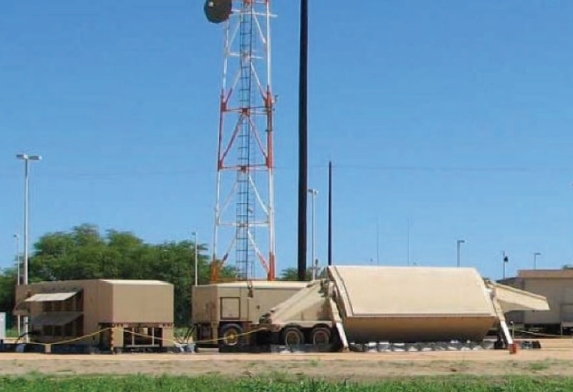
\includegraphics[width=1.0in]{figs/TRK_JPDAF_example_THAAD.jpg}
				\caption {THAAD, \\Theater High Altitude Area Defense)}
			}
			\end{figure}
		\end{column}
		\begin{column}{1.0in}
			\begin{figure}
			{
				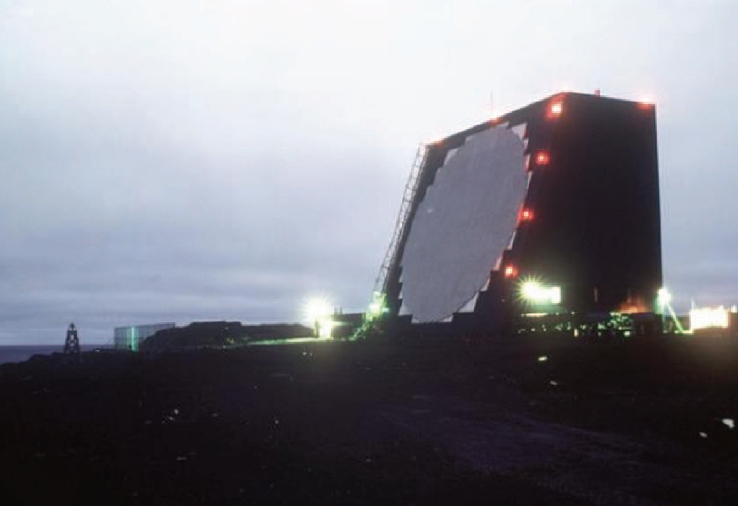
\includegraphics[width=1.0in]{figs/TRK_JPDAF_example_Cobra.jpg}
				\caption {Cobra Dane,\\long-range surveillance against ICBMs}
			}
			\end{figure}
		\end{column}
		\begin{column}{1.0in}
			\begin{figure}
			{
				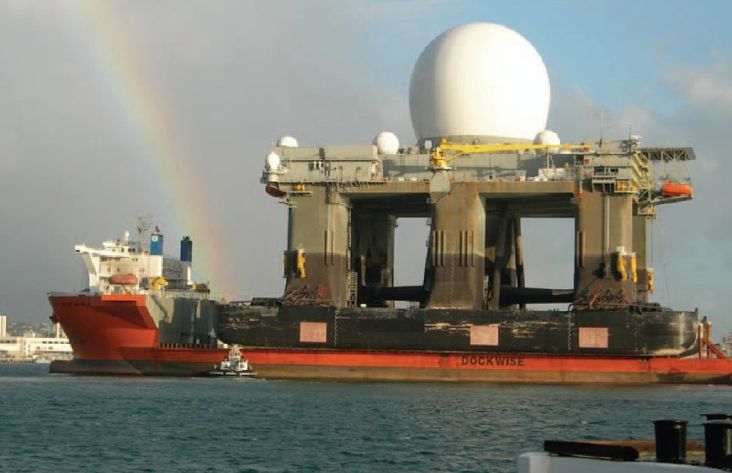
\includegraphics[width=1.0in]{figs/TRK_JPDAF_example_SBX.jpg}
				\caption {SBX,\\long-range surveillance against ICBMs}
			}
			\end{figure}
		\end{column}
	\end{columns}
\end{frame}



%------------------------------------------------------------
\subsubsection{\ \ \ \ \ \ \ \ MHT }
%------------------------------------------------------------
\begin{frame}
\frametitle{Multi-hypothesis tracker}
\logoCSIPCPL\mypagenum
	\begin{enumerate}
	\item {\color{red}Clustering}
		\begin{itemize}
			\item A new measurement is associated with a cluster if it falls within the validation region of any target within the cluster
		\end{itemize}
	\item {\color{red}Hypothesis Generation}
		\begin{itemize} 
			\item New hypotheses are generated for the measurements associated with each cluster
			\item The probability of each hypothesis is calculated
			\item Target estimates are then updated
		\end{itemize}
	\item {\color{red}Reduction}
		\begin{itemize}
			\item In this step, hypotheses are combined or eliminated
		\end{itemize}
	\item {\color{red}Simplify hypothesis matrix}
		\begin{itemize}
			\item Targets that are uniquely associated are removed from the hypothesis matrix
		\end{itemize}
	\end{enumerate}
\end{frame}




\begin{frame}
\frametitle{MHT}
\framesubtitle{usage}
\logoCSIPCPL\mypagenum
	MHT + EKF:
	\begin{figure}
		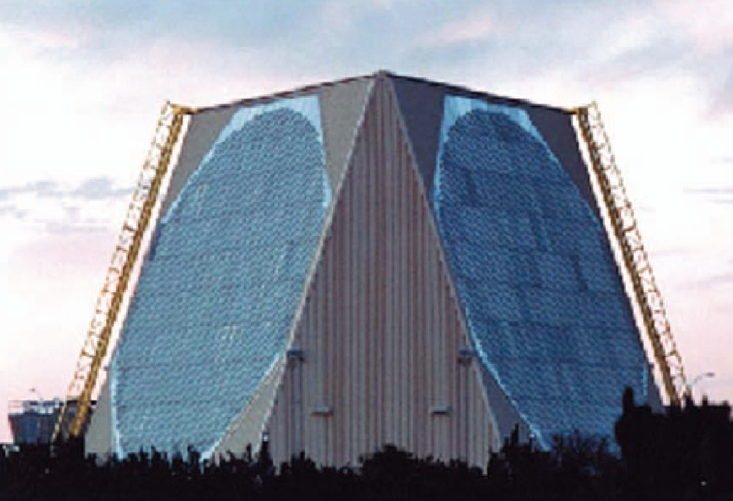
\includegraphics[width=0.7\textwidth]{figs/TRK_MHT_example_UEWR.jpg}
		\caption {UEWR, Upgraded Early Warning Radar, long-range surveillance against ICBMs}
	\end{figure}
\end{frame}


%#######################################################################
\section{III. Tracking: computer vision}
%#######################################################################


\begin{frame}
\frametitle{Pre-processing}
\logoCSIPCPL\mypagenum
	{\color{red}Steps}
	\begin{enumerate}
		\item Downsampling
		\item Normalization
		\item Stabilization
		\item Background modeling
		\item Feature Extraction
	\end{enumerate}
	\vspace{0.3in}
	{\color{red}Features}
	\begin{enumerate}
		\item Color
		\item Edges
		\item Corners
		\item Motion
		\item Texture
		\item Depth
		\item Density
	\end{enumerate}
\end{frame}


\begin{frame}
\frametitle{Background modeling}
\logoCSIPCPL\mypagenum
	\begin{figure}		
		\centering		
		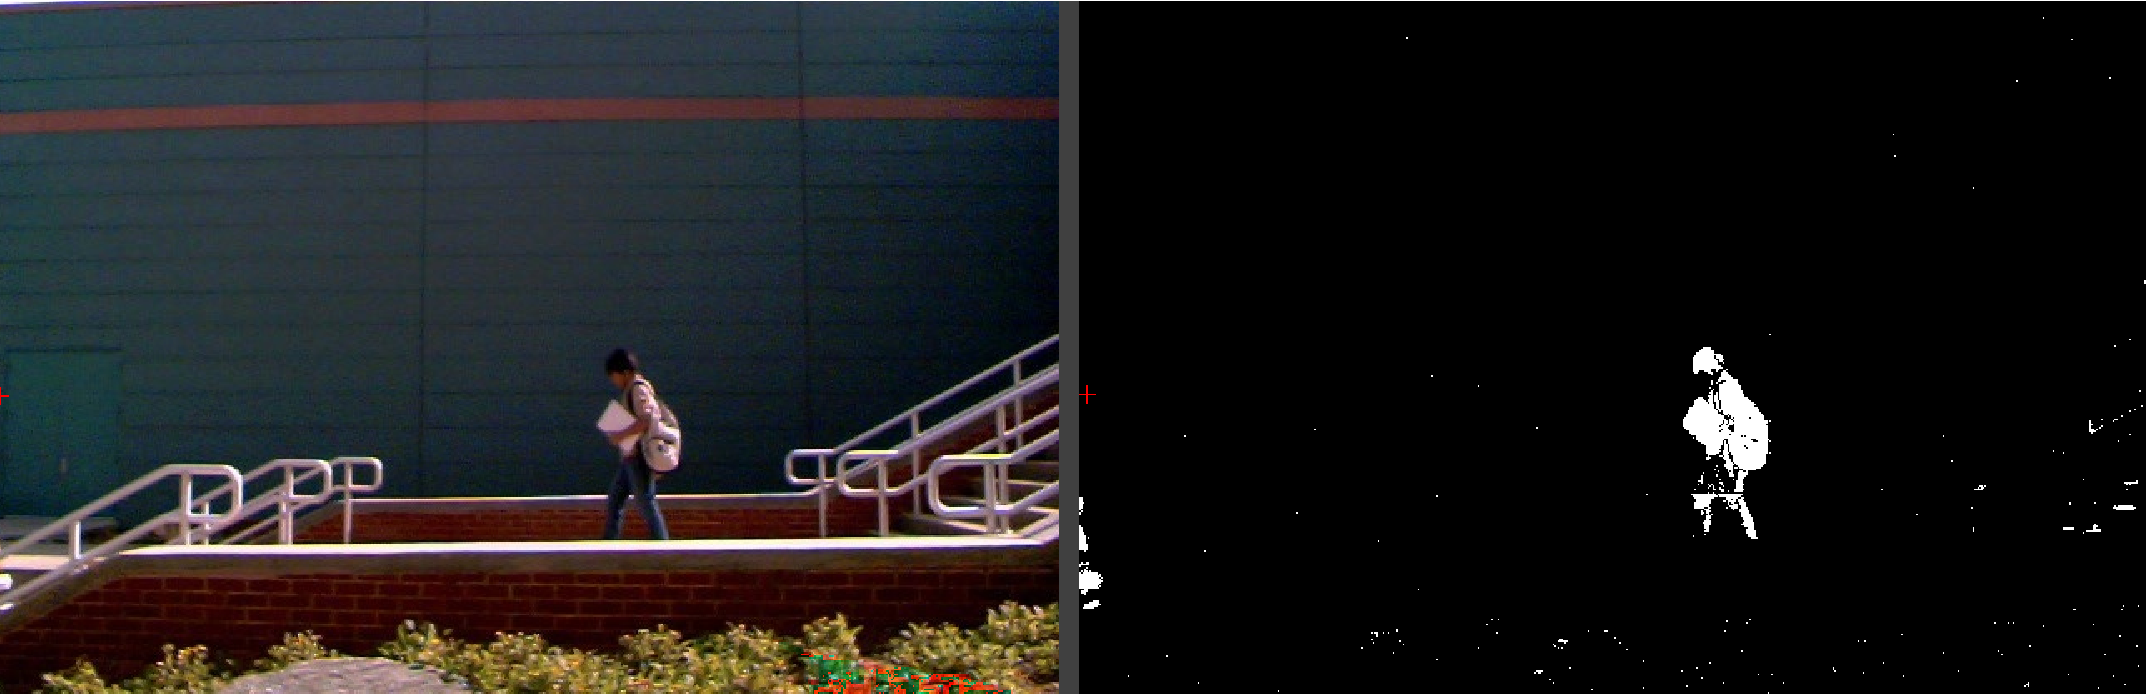
\includegraphics[width=1.0\textwidth]{figs/Proposal_fig12_TRK_multiGaussian.pdf}
		\label{fig:MultiGaussian}
	\end{figure}
\end{frame}


\begin{frame}
\frametitle{Color}
\framesubtitle{detection}
\logoCSIPCPL\mypagenum
	\begin{figure}		
		\centering		
		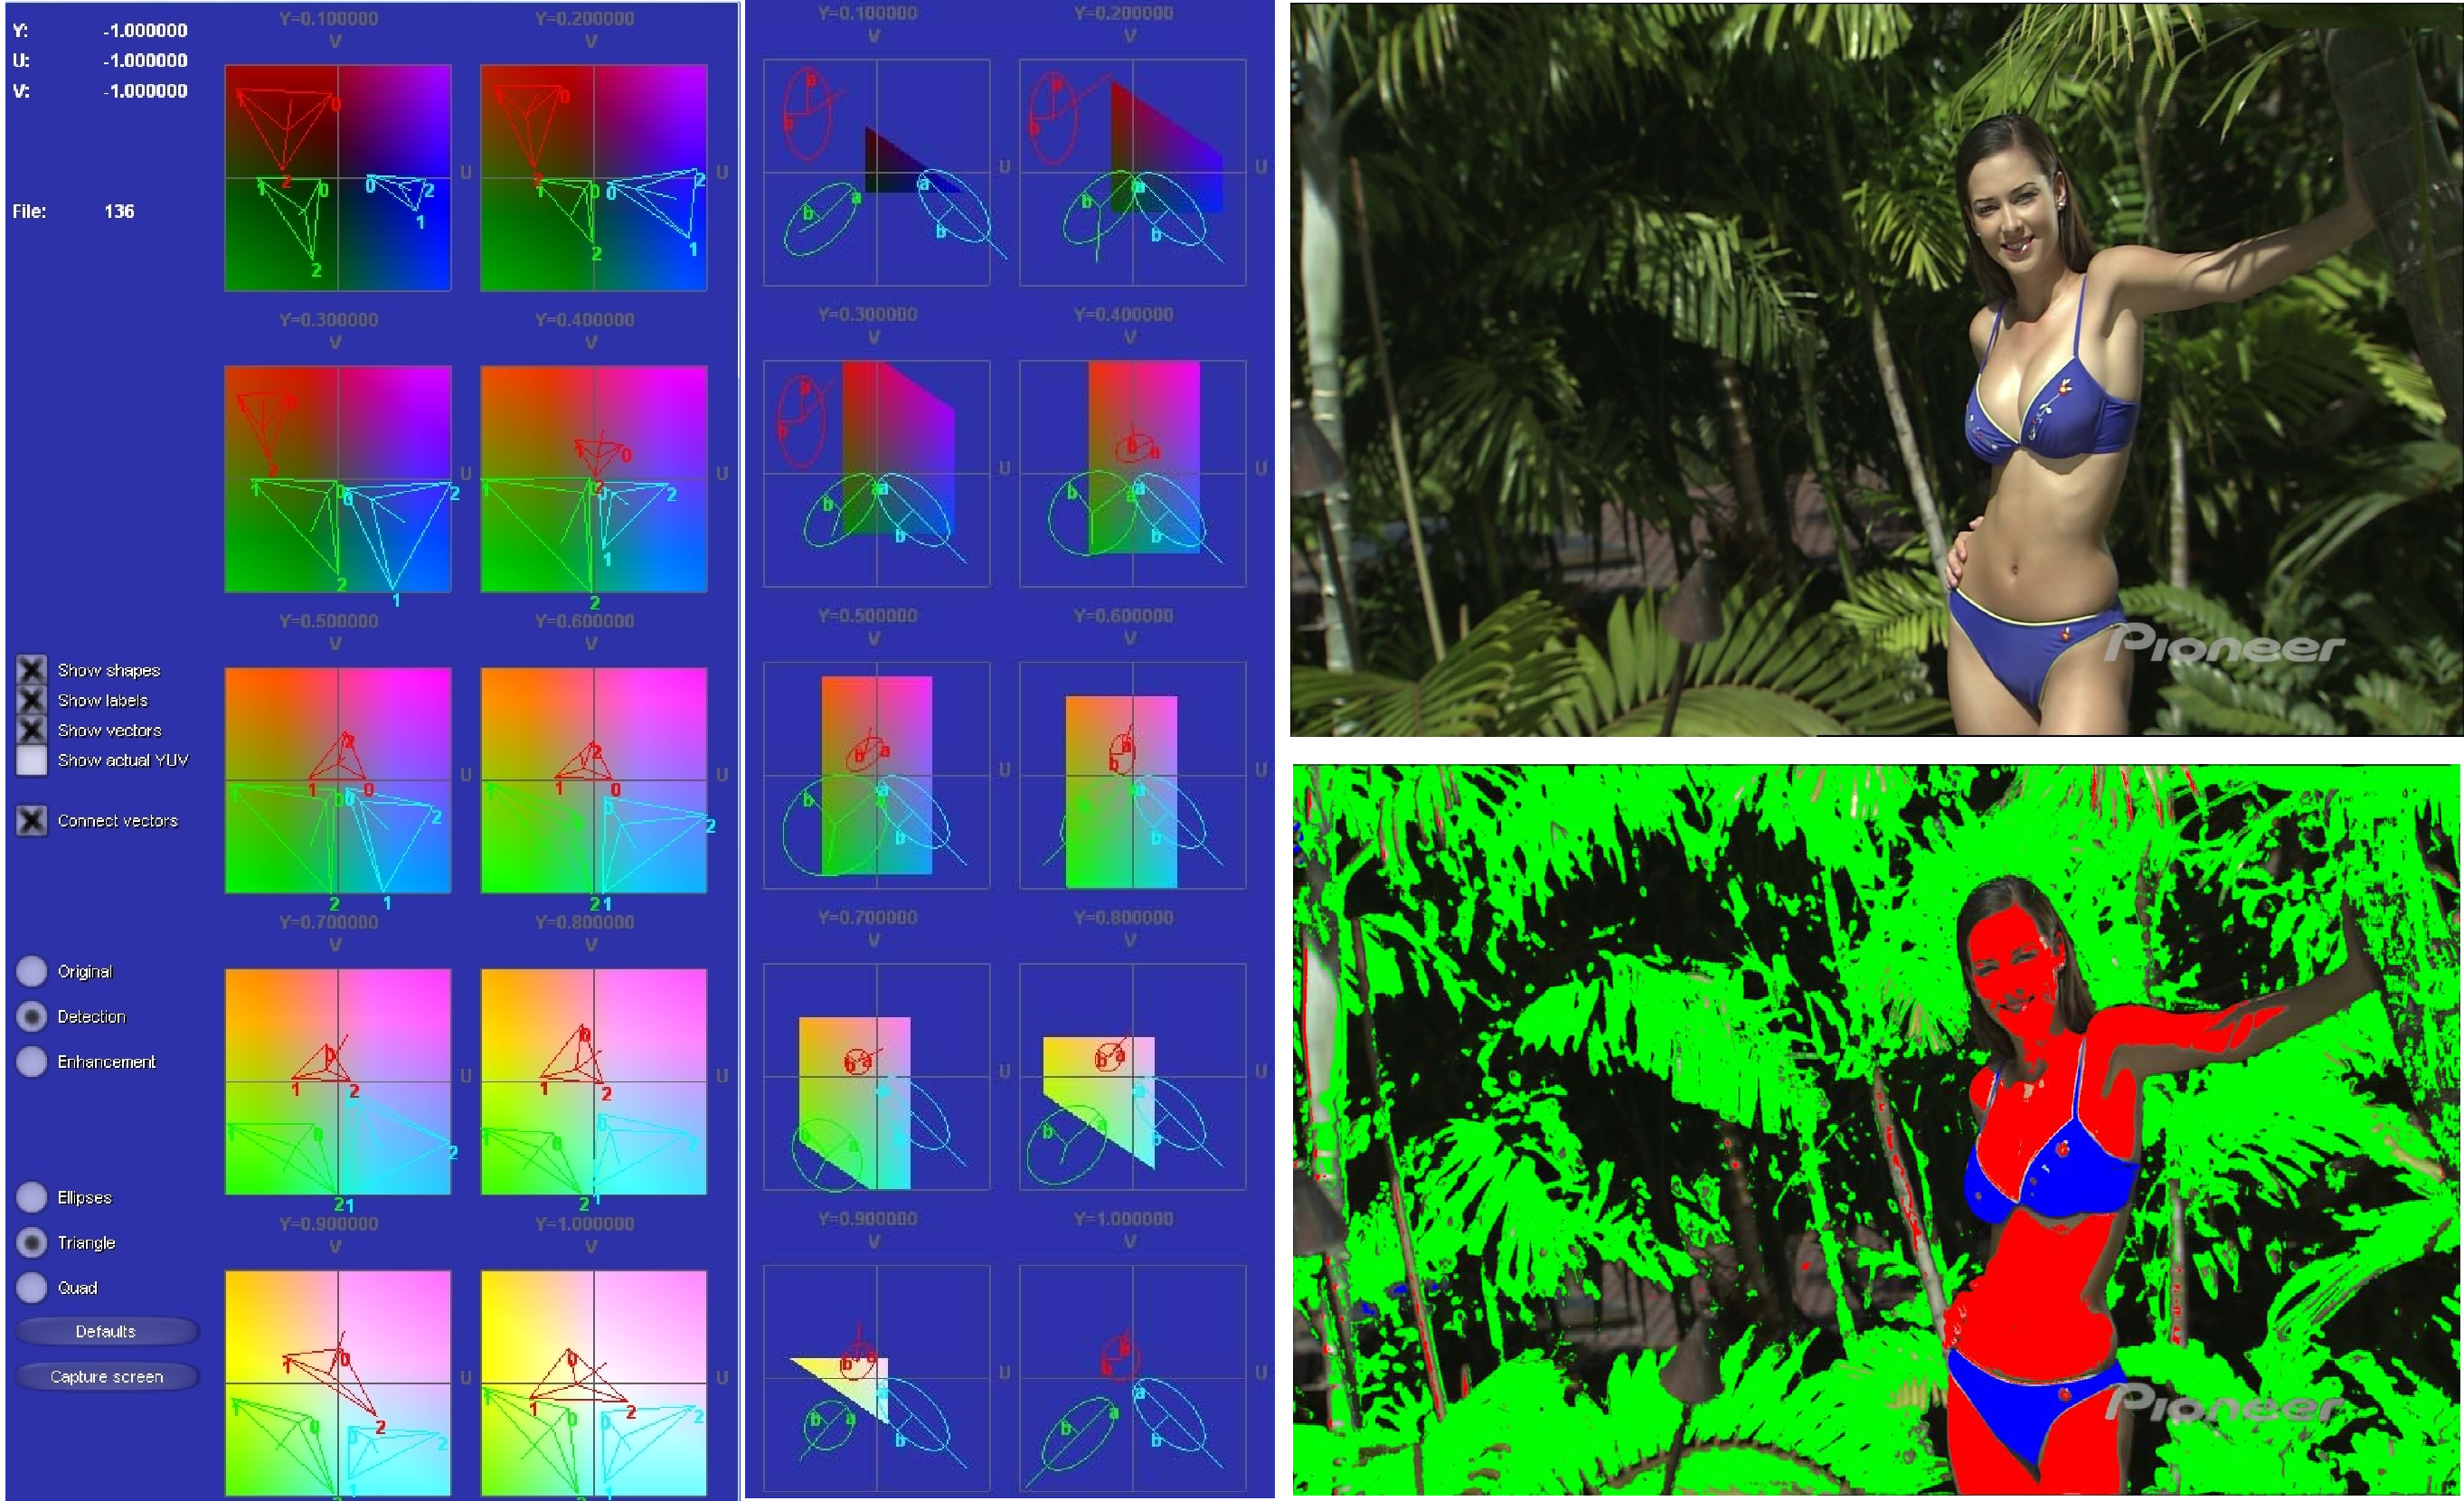
\includegraphics[width=1.0\textwidth]{figs/Proposal_fig14_TRK_colorDetection.pdf}
		\label{fig:color_detection}
	\end{figure}
\end{frame}


\begin{frame}
\frametitle{Color}
\framesubtitle{enhancement}
\logoCSIPCPL\mypagenum
	\begin{figure}		
		\centering		
		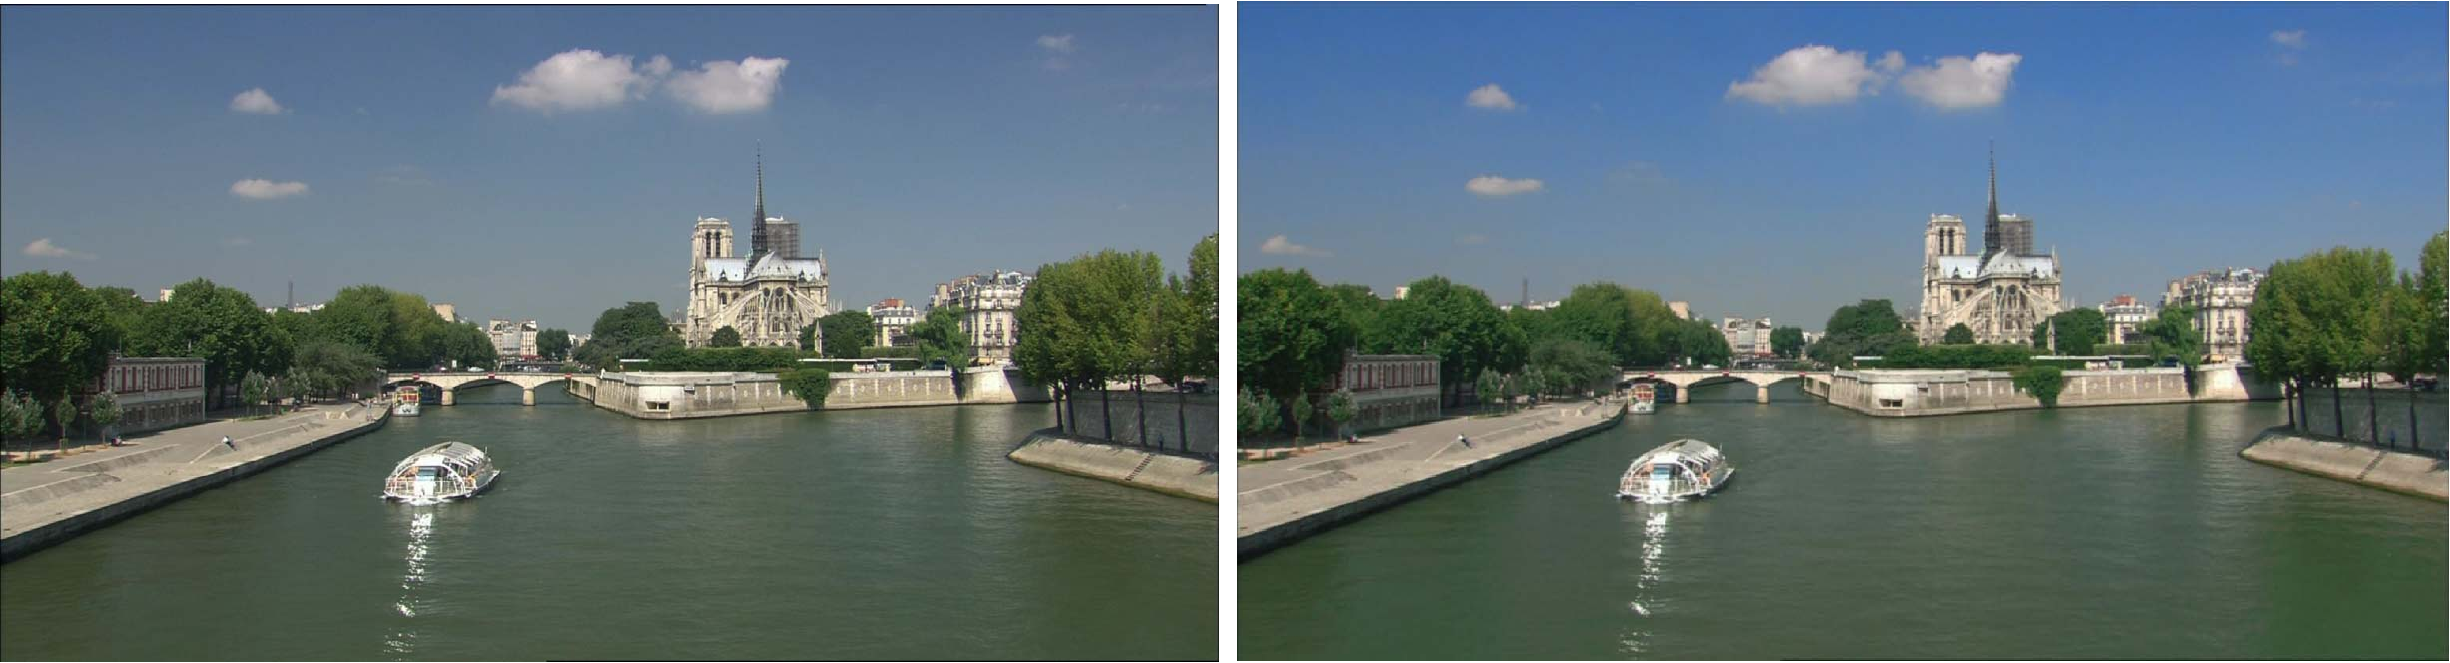
\includegraphics[width=1.0\textwidth]{figs/Proposal_fig15_TRK_colorEnhancement.pdf}
		\caption{Color enhancement}
		\label{fig:color_enhancement}
	\end{figure}
\end{frame}

\begin{frame}
\frametitle{Density}
\framesubtitle{Mean shift filtering: adaptive gradient ascent}
\logoCSIPCPL\mypagenum
	\begin{figure}				
		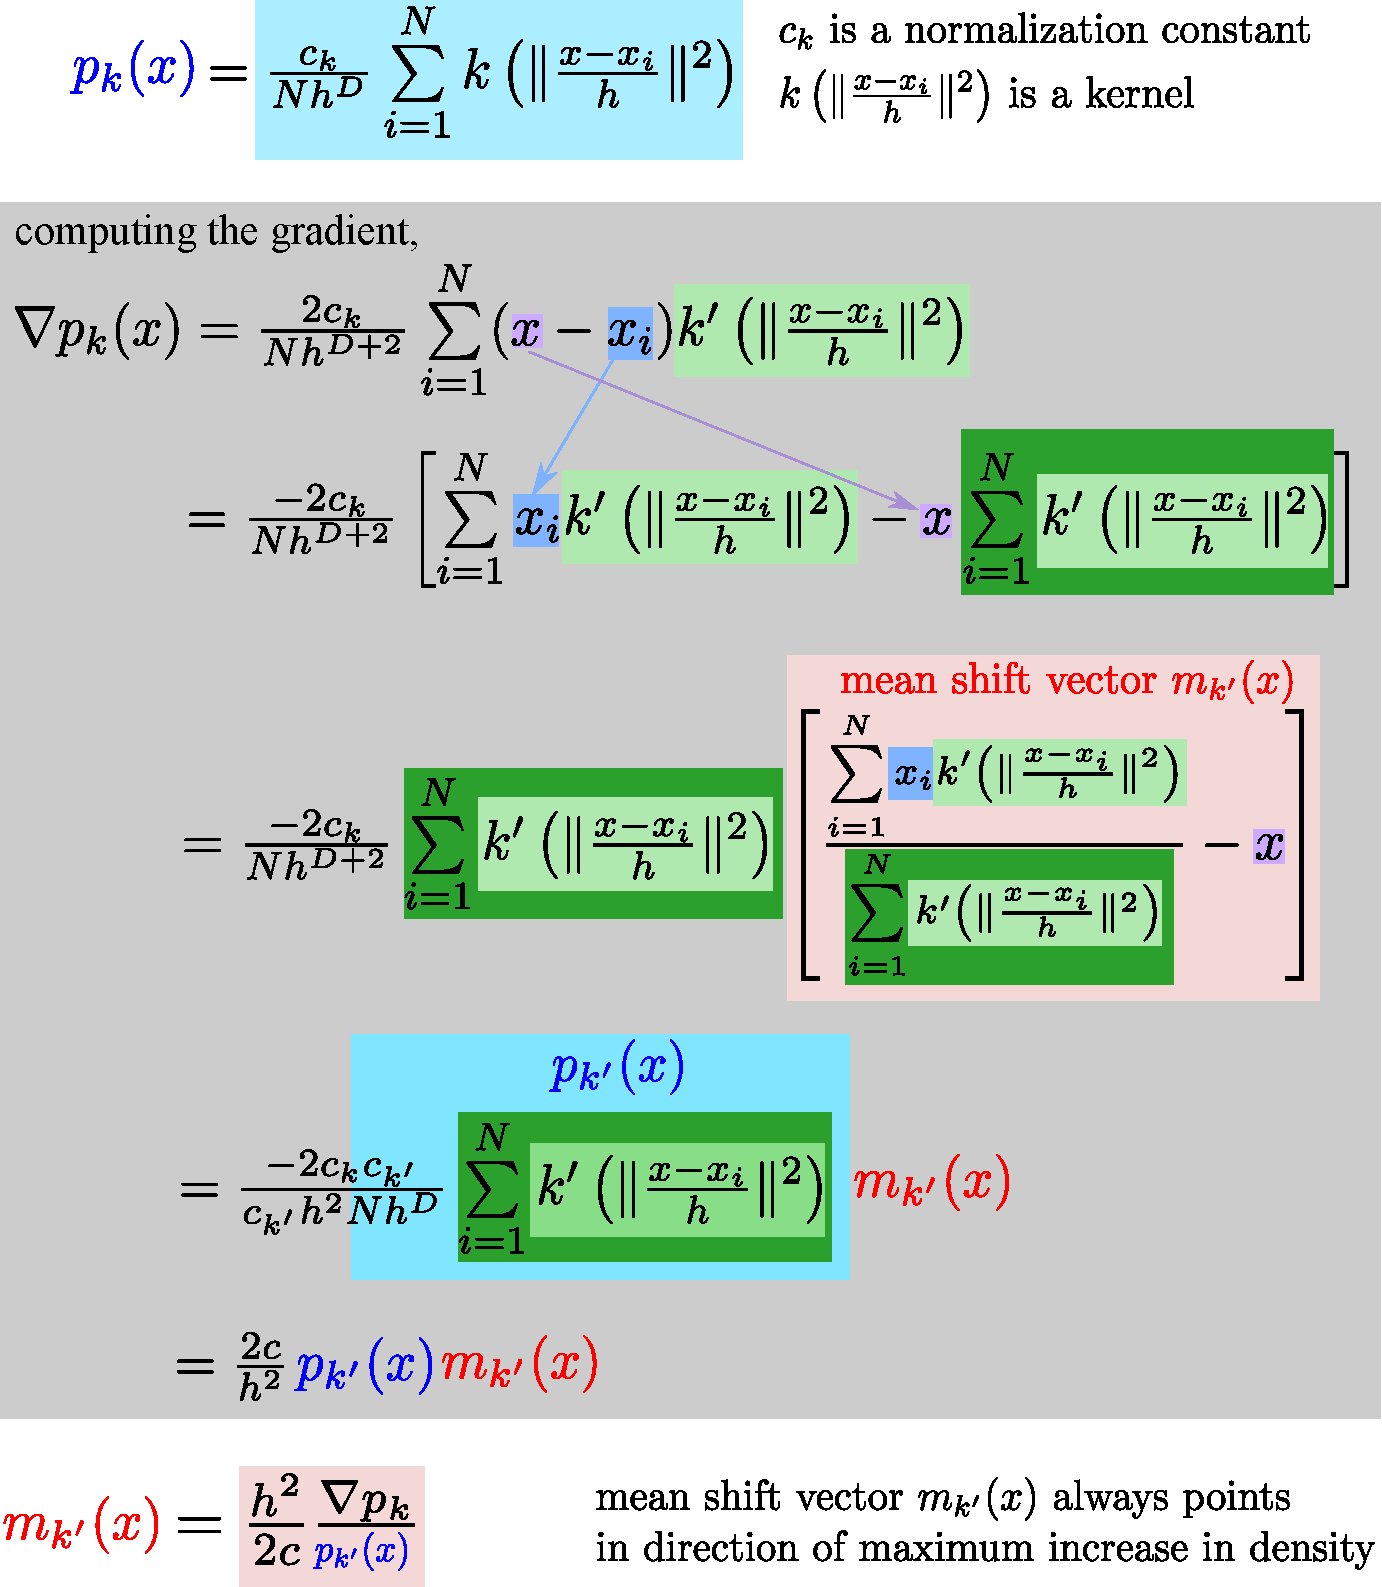
\includegraphics[height=.85\textheight]{figs/PRML_meanShift.pdf}
	\end{figure}
\end{frame}



\begin{frame}[plain]
\frametitle{Stereo}
\framesubtitle{depth}
\mypagenum
	\begin{changemargin}{-1.3in}{0in}
		\begin{figure}		
			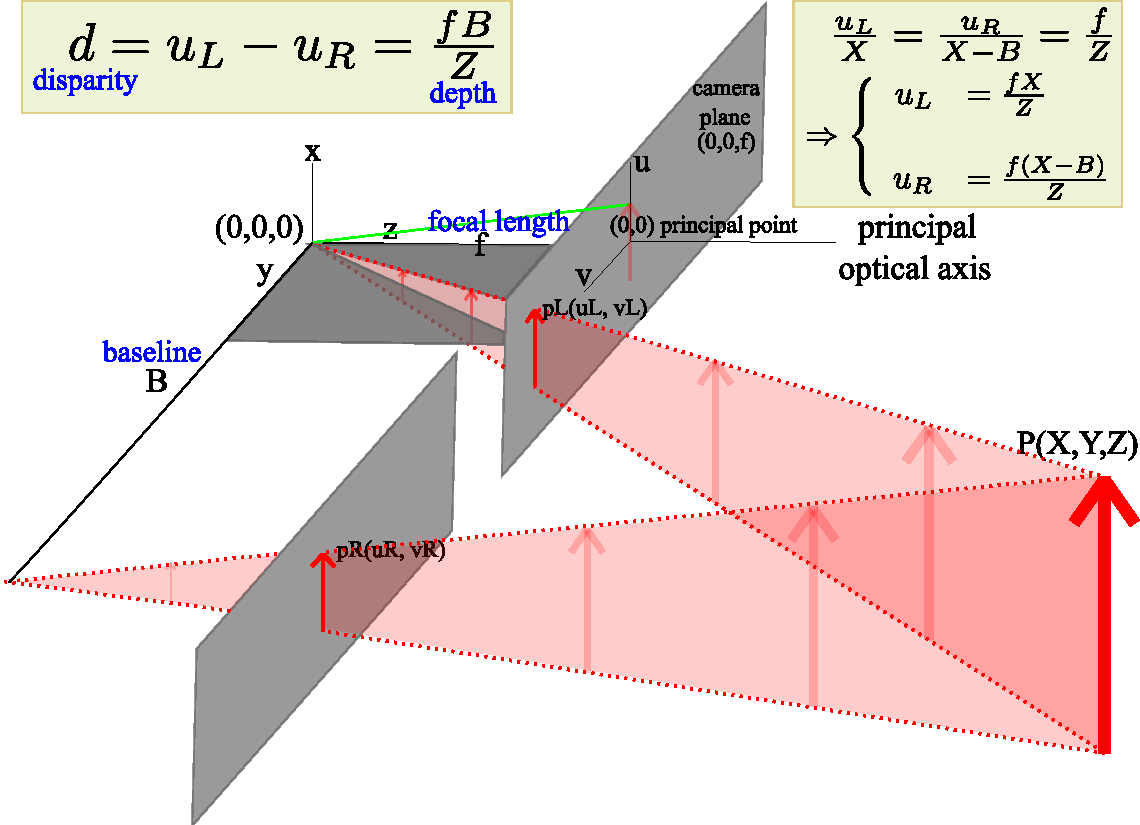
\includegraphics[width=1.3\textwidth]{figs/3D_2_cameras_blockDiagram.pdf}
		\end{figure}
	\end{changemargin}
\end{frame}	


%===================================================
\subsection{\ \ \ \ point}
%===================================================
\begin{frame}
\frametitle{Deterministic methods}
\framesubtitle{constraints}
\logoCSIPCPL\mypagenum
	\begin{itemize}
		\item proximity
		\item max velocity
		\item path coherence
			\begin{itemize}
				\item no abrupt motion change
			\end{itemize}
		\item motion smoothness
			\begin{itemize}
				\item path coherence over long durations
			\end{itemize}			
		\item rigidity
	\end{itemize}
\end{frame}


\begin{frame}
\frametitle{Particle Filter}
\framesubtitle{multi-modal PDF}
\logoCSIPCPL\mypagenum
	\begin{figure}
		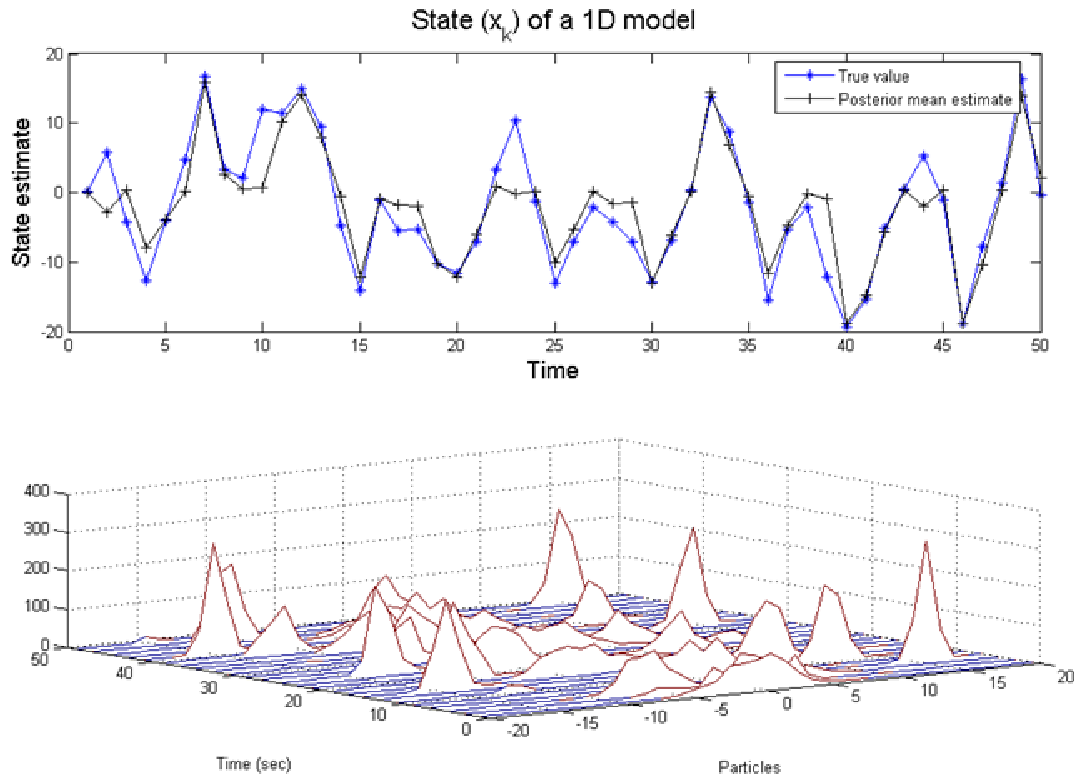
\includegraphics[width=1.0\textwidth]{figs/TRK_ParticleFilter_multimodalPDF.pdf}
	\end{figure}	
\end{frame}




%\begin{frame}
%\frametitle{Particle Filter}
%\framesubtitle{weight update}
%\logoCSIPCPL\mypagenum
%	\begin{figure}
%		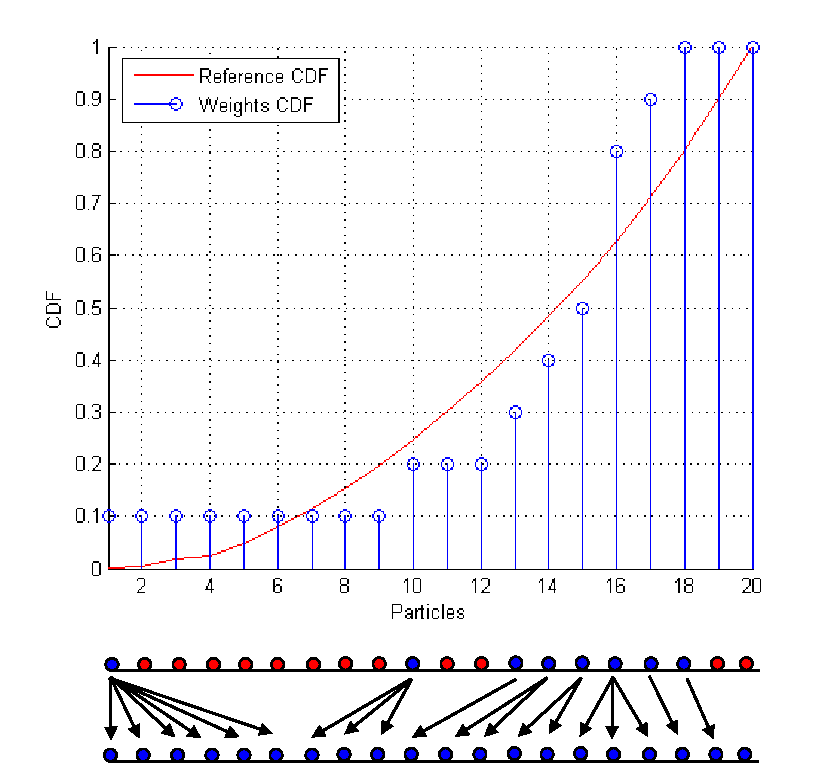
\includegraphics[width=0.9\textwidth]{figs/TRK_ParticleFilter_weightUpdates.pdf}
%	\end{figure}	
%\end{frame}

%===================================================
\subsection{\ \ \ \ region}
%===================================================
\begin{frame}
\frametitle{Region tracking}
\framesubtitle{overview}
\logoCSIPCPL\mypagenum
	\begin{enumerate}
		\item Template matching
			\begin{itemize}
				\item fixed templates: reliable over short durations \href{run:distribute/run_TRK_templateMatching.bat}{{\color{blue}\underline {demo}}}
			\end{itemize}
		\item Subspace methods
			\begin{itemize}
				\item usually learned with PCA
				\item model variations in lighting and pose
				\item disadvantages: object specific, training
			\end{itemize}			
		\item Probability density
			\begin{itemize}
				\item robustness under image distortions and occlusions
				\item fast to learn
				\item disadvantage: lack of expressiveness, registration can be difficult
			\end{itemize}
		\item Motion
			\begin{itemize}
				\item optical flow works well for small displacements
				\item block matching for large motion
				\item computing motion vectors is computationally complex
			\end{itemize}
	\end{enumerate}
\end{frame}





%\begin{frame}
%\frametitle{Mean shift tracking on compressed video}
%\framesubtitle{goal}
%\logoCSIPCPL\mypagenum
%	We want to run some computer vision algorithm (e.g. tracking) on compressed video.
%	\begin{itemize}
%		\item We would like the results of the algorithm (e.g. track positions) to be as close as possible to results generated if the algorithm were run on uncompressed video.
%	\end{itemize}
%	\begin{figure}		
%		\includegraphics[width=0.9\textwidth]{figs/ICIP2009_ProblemStatement.pdf}
%	\end{figure}
%\end{frame}



\begin{frame}
\frametitle{Mean shift tracking}
\framesubtitle{solutions for compressed video}
\logoCSIPCPL\mypagenum
	\begin{figure}		
		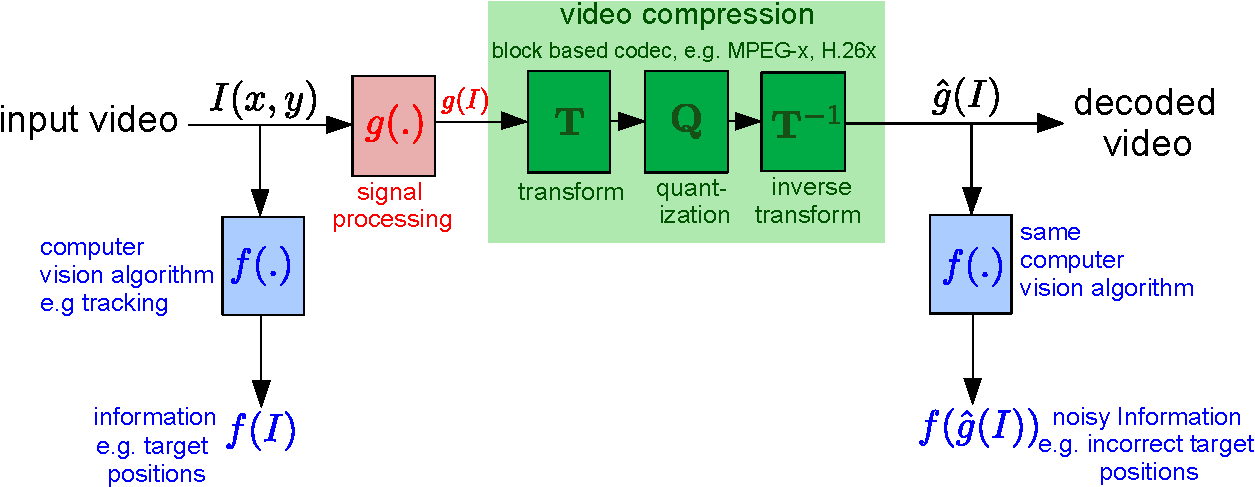
\includegraphics[width=1.0\textwidth]{figs/ICIP2009_SolutionThroughSigProc.pdf}
	\end{figure}
	\begin{figure}
		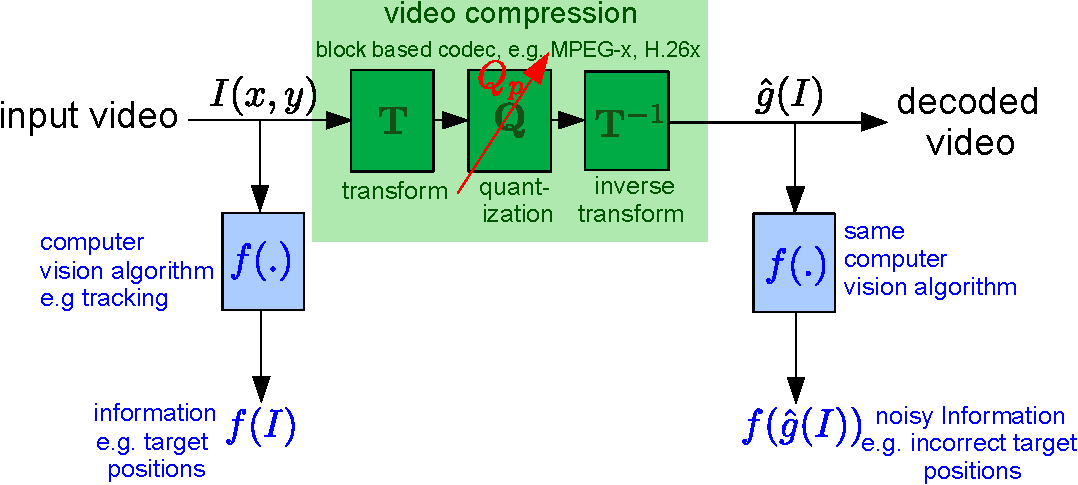
\includegraphics[width=0.9\textwidth]{figs/TRK_IPCV2009_BlockDiagram_2_VarPar_2.pdf}
	\end{figure}
\end{frame}




\begin{frame}
\frametitle{Mean shift tracking}
\framesubtitle{Compressed video results, PETS2001 \tiny{\footnote{S. M. Aslam, A. F. Bobick, and C. F. Barnes, Better computer vision under video compression, an example using mean shift tracking," in \emph{IEEE International Conference on Image Processing, 2009}.}}} 
\logoCSIPCPL\mypagenum
	\begin{itemize}
		\item person tracking
		\item sparse background
		\item target occluded by object (car) with similar color distribution
	\end{itemize}
	\begin{figure}
		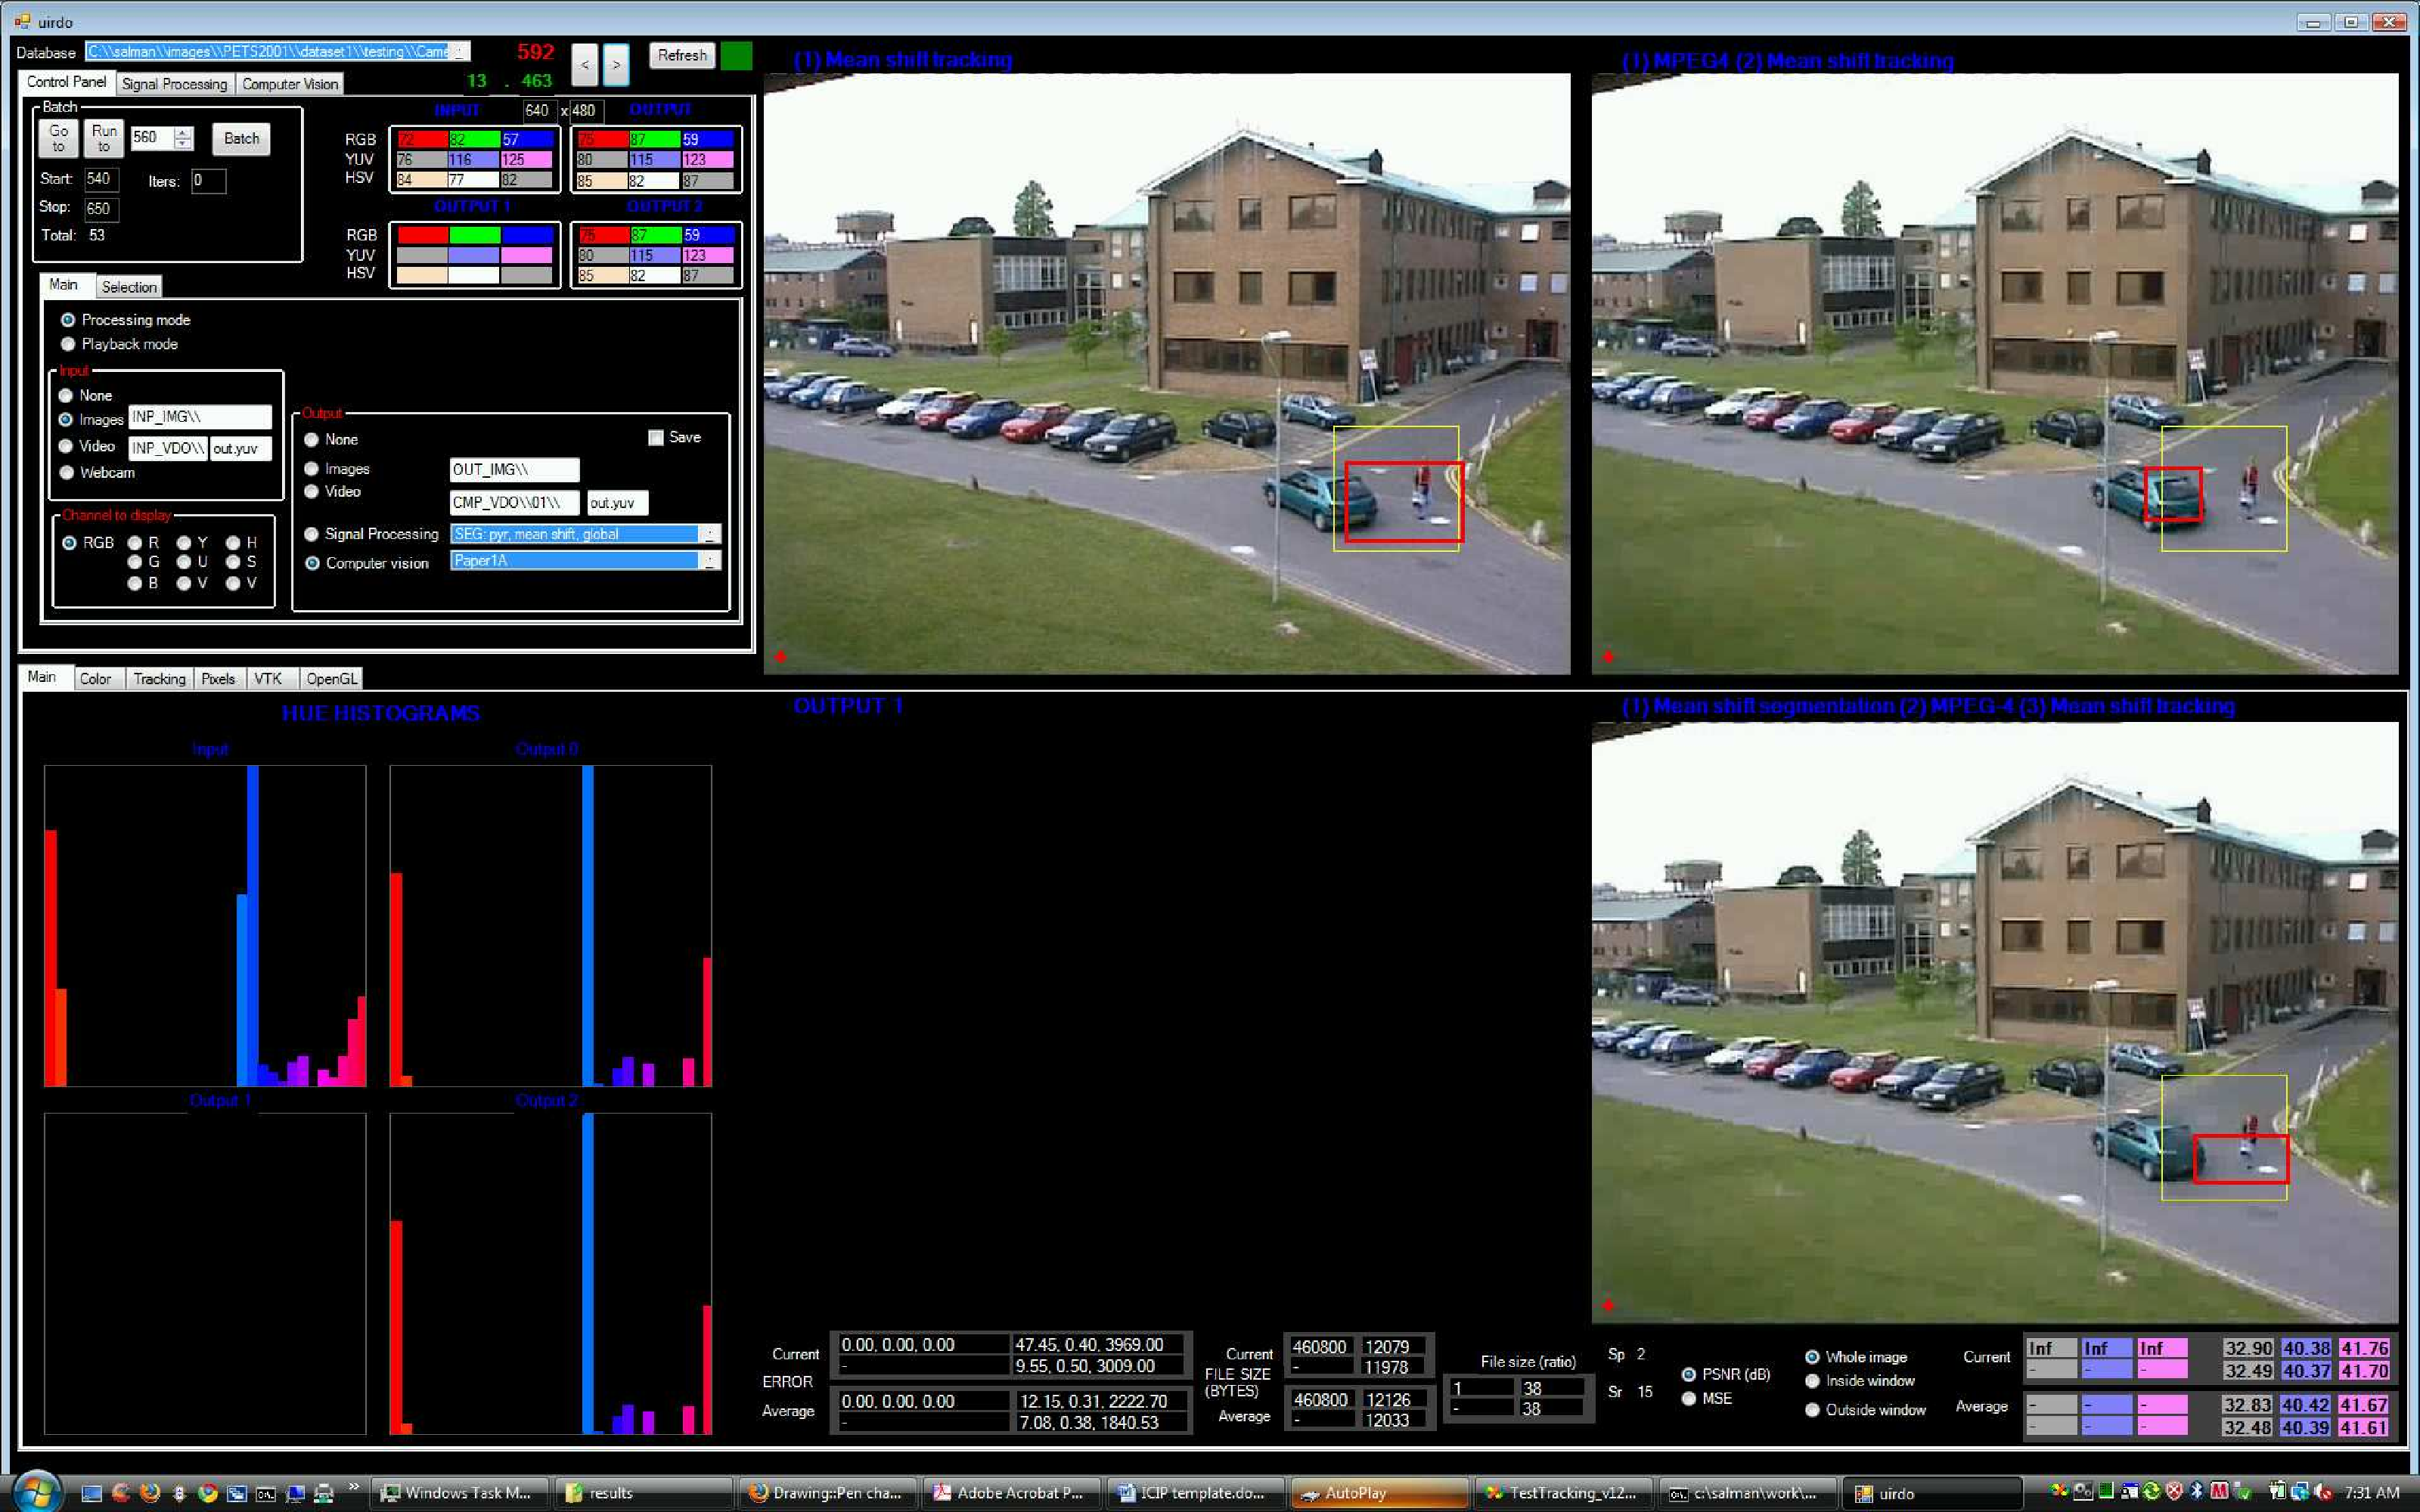
\includegraphics[width=0.8\textwidth]{figs/ICIP2009_PETS2001_FN_00592_snapshotVVG.pdf}
	\end{figure}
\end{frame}


\begin{frame}
\frametitle{Mean shift tracking}
\framesubtitle{Compressed video results, PETS2001 (cont.)} 
\logoCSIPCPL\mypagenum
	\begin{figure}
		\centering
		\subfigure[Ground truth]
			{
				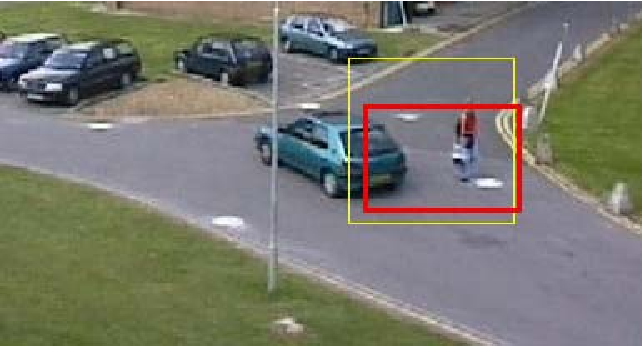
\includegraphics[width=.45\textwidth]{figs/TRK_IPCV2009_PETS2001_FN_00592_outputGroundTruth}
				\label{fig:PETS2001_Frame592_Ground}
			}
		\subfigure[Base]
			{
				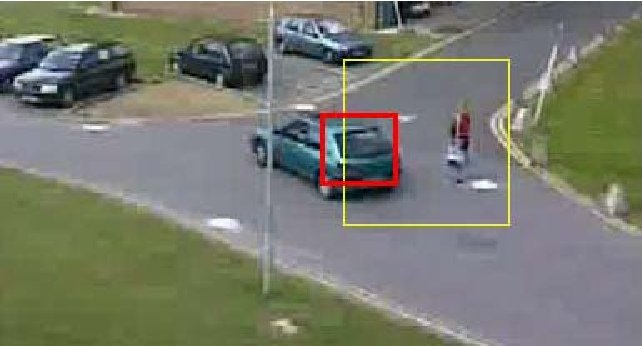
\includegraphics[width=.45\textwidth]{figs/TRK_IPCV2009_PETS2001_FN_00592_outputBaseline}
				\label{fig:PETS2001_Frame592_Base}
			}
		\subfigure[SigProc]
			{
				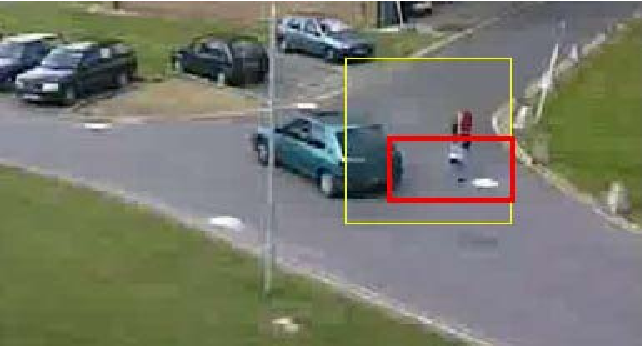
\includegraphics[width=.45\textwidth]{figs/TRK_IPCV2009_PETS2001_FN_00592_outputSigProc}
				\label{fig:PETS2001_Frame592_SigProc}
			}
		\subfigure[VarPar]
			{
				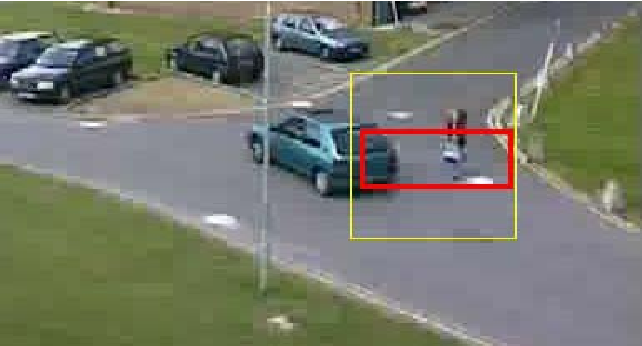
\includegraphics[width=.45\textwidth]{figs/TRK_IPCV2009_PETS2001_FN_00592_outputVarPar}
				\label{fig:PETS2001_Frame592_VarPar}
			}	
	\end{figure}
\end{frame}





\begin{frame}
\frametitle{Mean shift tracking}
\framesubtitle{Compressed video results, PETS2007 } 
\logoCSIPCPL\mypagenum
	\begin{itemize}
		\item object (bag) tracking
		\item dense background
		\item target occluded by object with similar color distribution
	\end{itemize}
	\begin{figure}
		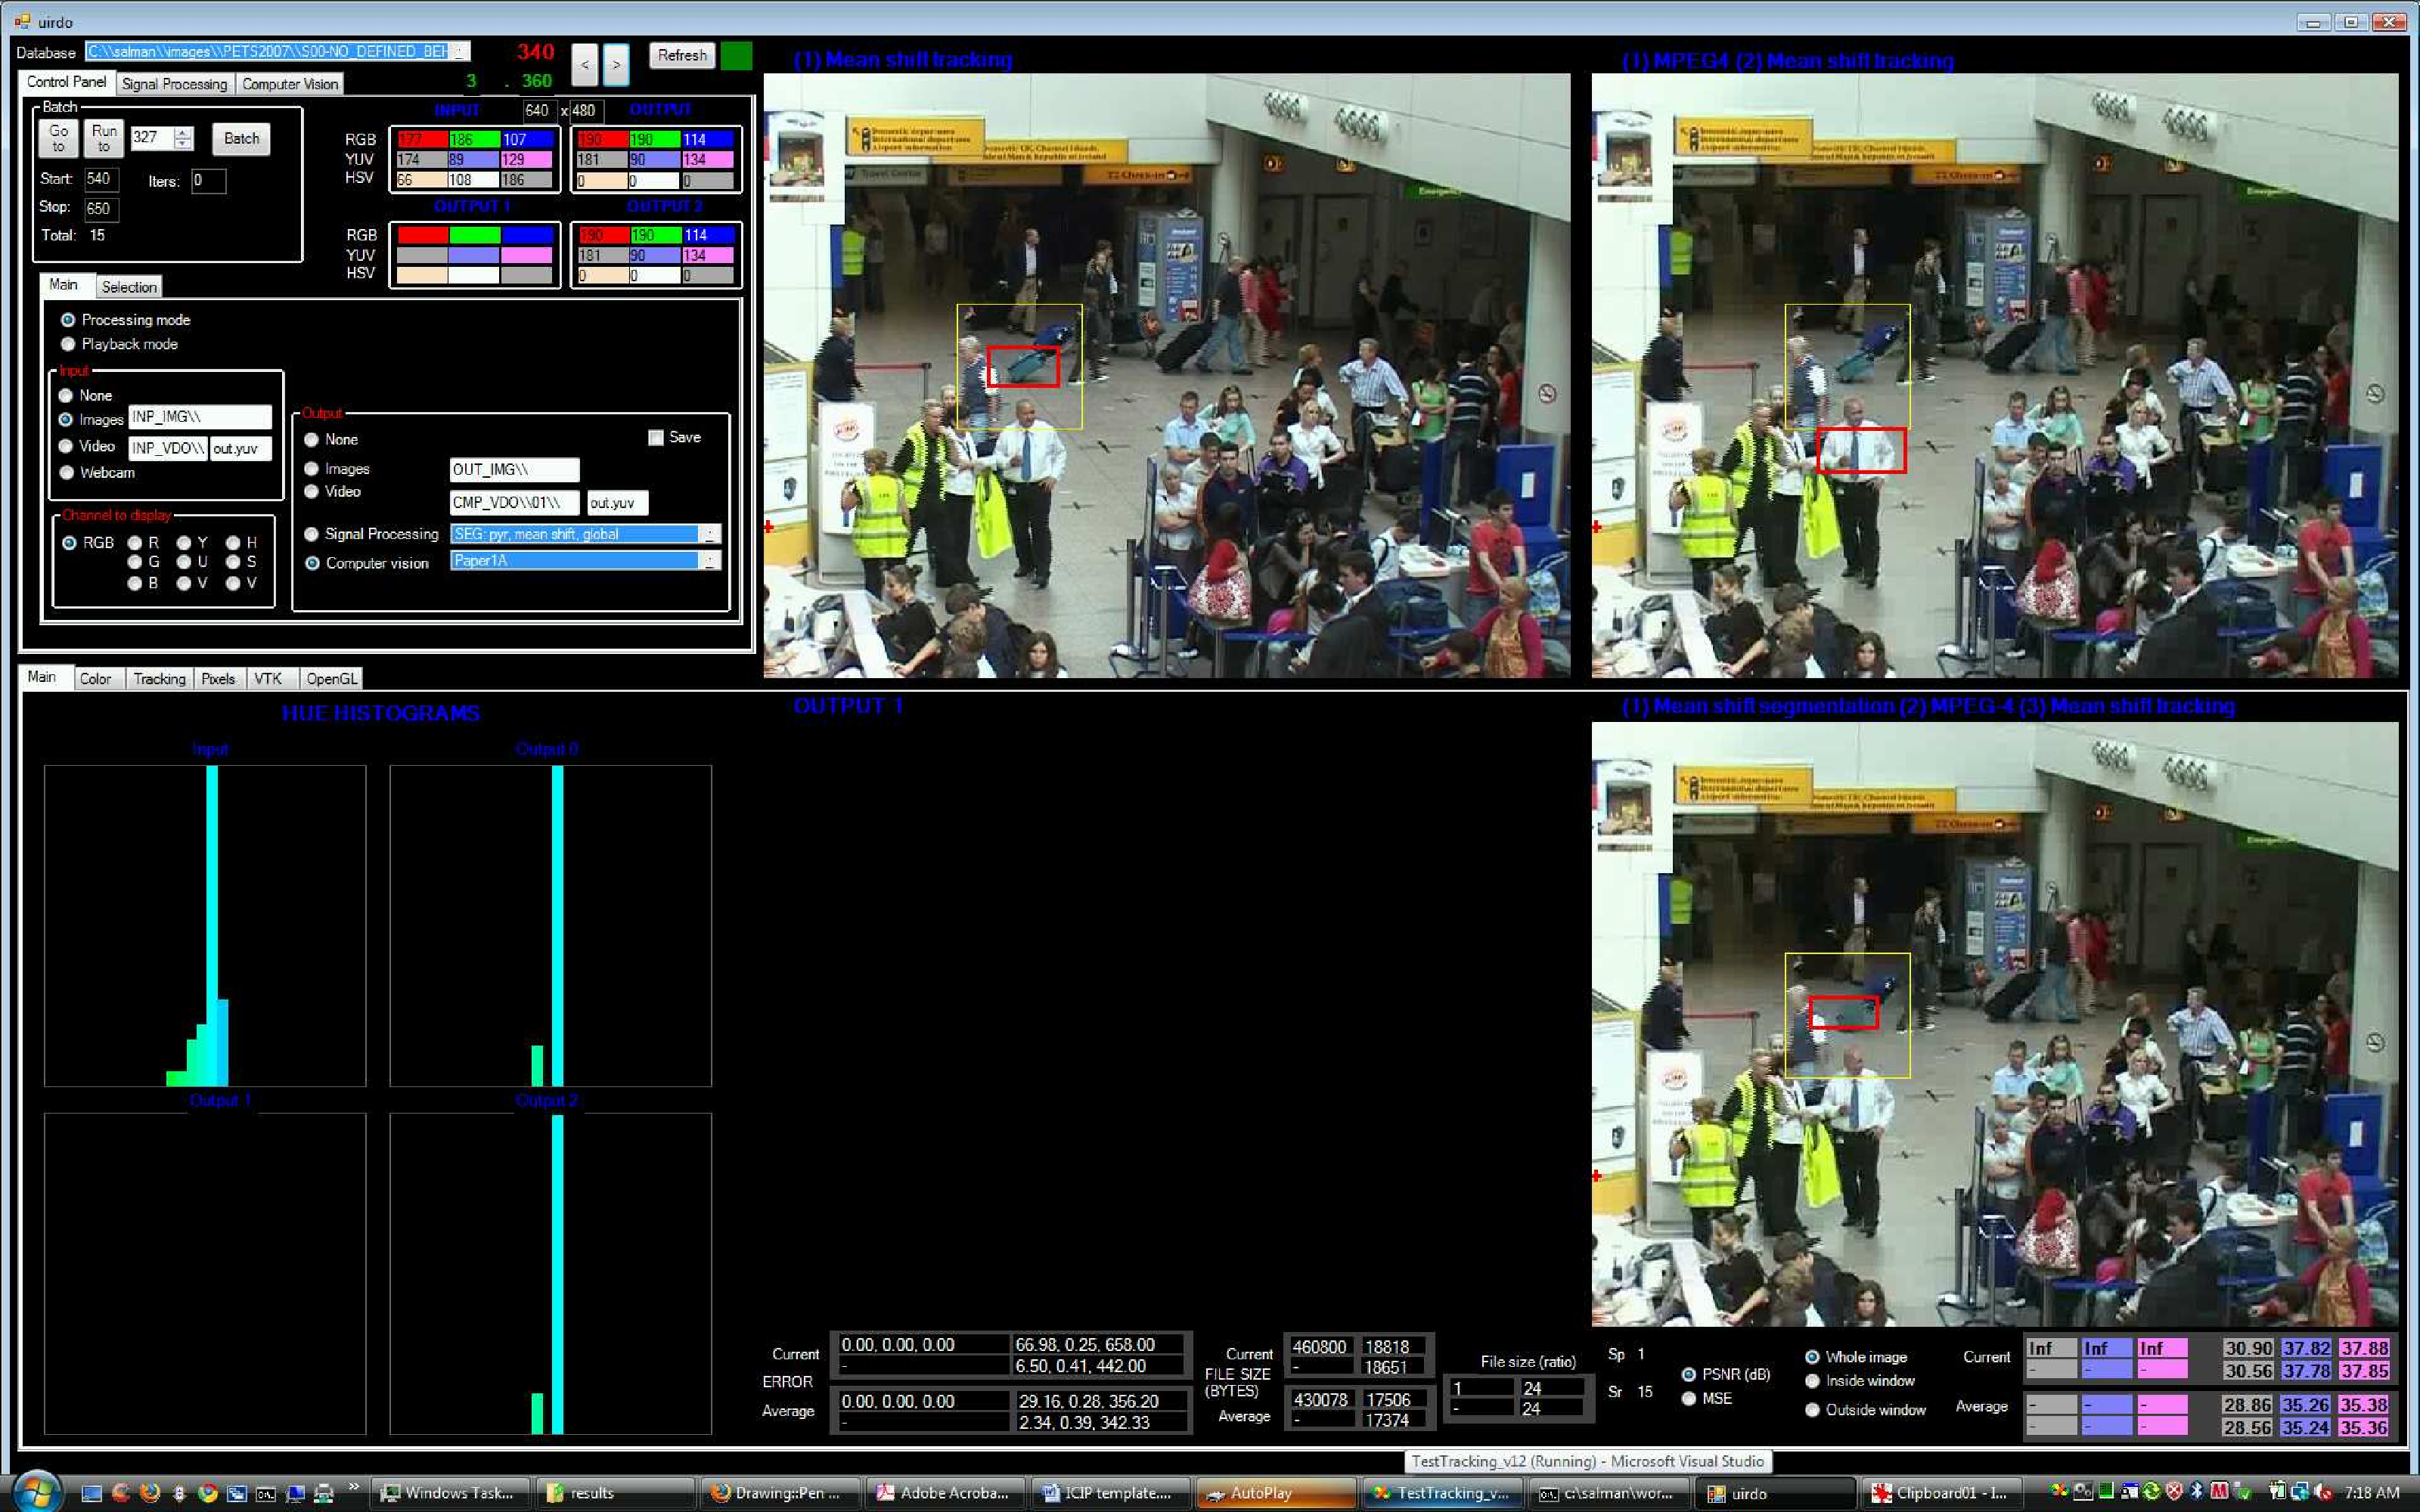
\includegraphics[width=1.0\textwidth]{figs/ICIP2009_PETS2007_FN_00340_snapshotVVG.pdf}
	\end{figure}
\end{frame}






\begin{frame}
\frametitle{Mean shift tracking}
\framesubtitle{Compressed video results, PETS2007 (cont.)} 
\logoCSIPCPL\mypagenum
	\begin{figure}%[htp]
		\centering
		\subfigure[Ground truth]
			{
				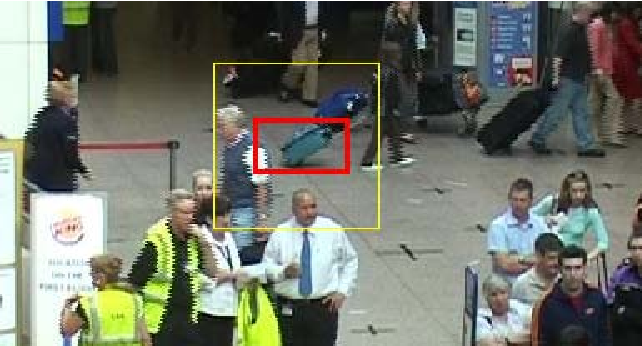
\includegraphics[width=.45\textwidth]{figs/TRK_IPCV2009_PETS2007_FN_00340_outputGroundTruth}
				\label{fig:PETS2007_Frame340_Ground}
			}
		\subfigure[Base]
			{
				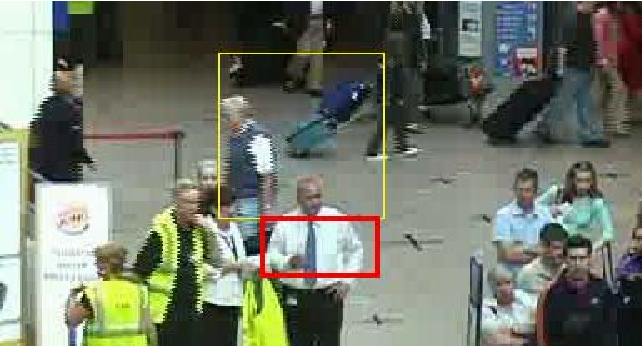
\includegraphics[width=.45\textwidth]{figs/TRK_IPCV2009_PETS2007_FN_00340_outputBaseline}
				\label{fig:PETS2007_Frame340_Base}
			}
		\subfigure[SigProc]
			{
				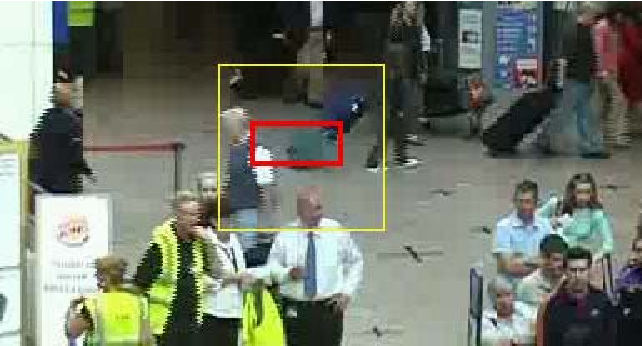
\includegraphics[width=.45\textwidth]{figs/TRK_IPCV2009_PETS2007_FN_00340_outputSigProc}
				\label{fig:PETS2007_Frame340_SigProc}
			}
		\subfigure[VarPar]
			{
				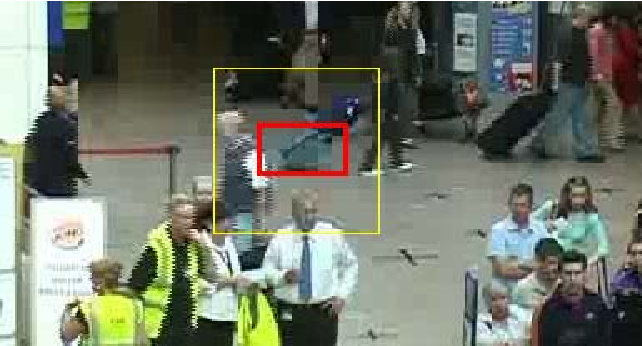
\includegraphics[width=.45\textwidth]{figs/TRK_IPCV2009_PETS2007_FN_00340_outputVarPar}
				\label{fig:PETS2007_Frame340_VarPar}
			}	
	\end{figure}
\end{frame}



%\begin{frame}
%\frametitle{Tracking error}
%\framesubtitle{plotted against $Q_p$ and time, 3D}
%\logoCSIPCPL\mypagenum
%	\begin{figure}
%		\centering
%		\subfigure[PETS2001]
%		{	
%			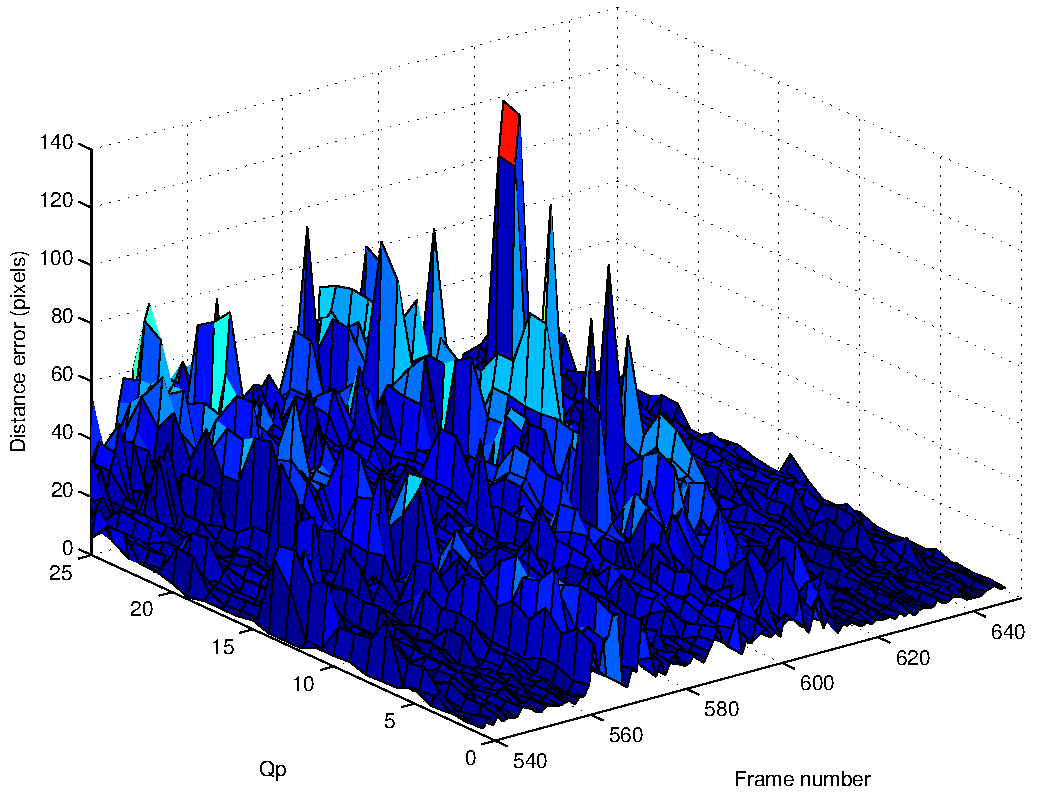
\includegraphics[width=.45\textwidth]{figs/TRK_IPCV2009_PETS2001_TrackingError3D}
%		}
%		\subfigure[PETS2007]
%		{	
%			\includegraphics[width=.45\textwidth]{figs/TRK_IPCV2009_PETS2007_TrackingError3D}
%		}
%		\caption{$VarPar$, tracking accuracy at different values of $Qp$.}
%	\end{figure}
%\end{frame}
%
%
%
%\begin{frame}
%\frametitle{Tracking error}
%\framesubtitle{plotted against $Q_p$ and time, 2D}
%\logoCSIPCPL\mypagenum
%	\begin{figure}
%		\centering
%		\subfigure[PETS2001]
%			{
%				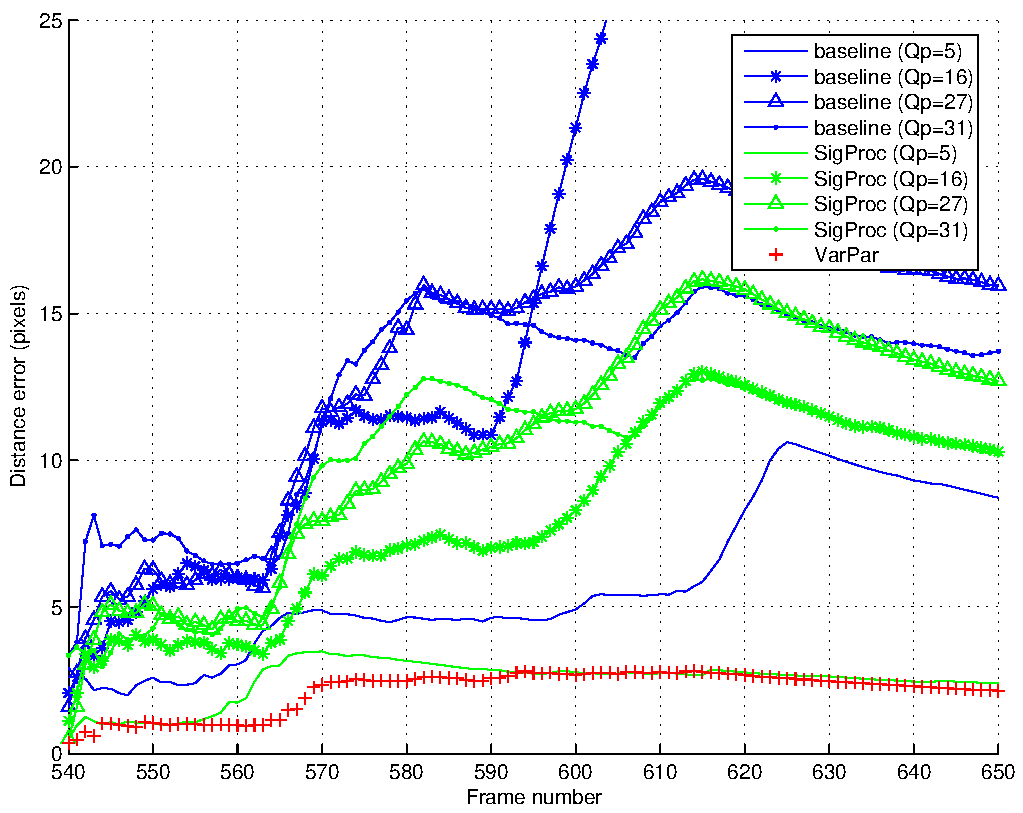
\includegraphics[width=.45\textwidth]{figs/TRK_IPCV2009_PETS2001_TrackingError}
%			}
%		\subfigure[PETS2007]
%			{
%				\includegraphics[width=.45\textwidth]{figs/TRK_IPCV2009_PETS2007_TrackingError}
%			}
%	\end{figure}
%\end{frame}





%\begin{frame}
%\frametitle{Tracking error}
%\framesubtitle{average over time and datasets}
%\logoCSIPCPL\mypagenum
%	\begin{figure}
%		\includegraphics[width=1.0\textwidth]{figs/TRK_IPCV2009_TrackingErrorAllQp.pdf}
%	\end{figure}
%\end{frame}





\begin{frame}
\frametitle{Mean shift tracking}
\framesubtitle{Compressed video tracking error\tiny{\footnote{S. M. Aslam, C. F. Barnes, and A. F. Bobick, Compensation methods using signal processing and adaptive quantization for better mean shift tracking on compressed video," in \emph{International Conference on Image Processing, Computer Vision, and Pattern Recognition, 2009}.}}}
\logoCSIPCPL\mypagenum
	\begin{table}
		\centering
		\begin{tabular}{|l|c|c|c|c|}
			\hline
			\multicolumn{5}{|c|}{Accuracy (distance from ground truth)} \\
			\hline
			Dataset & Qp & Baseline & $SigProc$  & $VarPar$\\ 
			\hline
			\multirow{4}{*}{PETS2001} 
				&5  & 8.7 	&   2.4 &   2.1 \\
				&16 & 75.4 &  10.3 &   2.1\\
				&27 &16.0 	&  12.7 &   2.1\\
				&31 &13.7 &  10.2 &   2.1\\
			\hline
			\multirow{3}{*}{PETS2007} 
				&5 &5.8 &   3.5 &   1.0\\
				&16 &85.1 &   4.2 &   1.0\\
				&27 &71.8 &   3.5 &   1.0\\
				&31 &15.2 &  35.8 &   1.0\\
			\hline
			\multirow{1}{*}{Average}
			& - & 36.5 & 10.3 & 1.6 \\  
			\hline
		\end{tabular}
	\end{table}
\end{frame}



%===================================================
\subsection{\ \ \ \ contour}
%===================================================

%-------------------------------------------------
\subsubsection{\ \ \ \ \ \ \ \ \   representation}
%-------------------------------------------------

\begin{frame}
\frametitle{Contour representation}
\framesubtitle{polynomials}
\logoCSIPCPL\mypagenum
	\begin{figure}
		\includegraphics[width=1.0\textwidth]{figs/theory_contour_PolynomialFitting.pdf}
	\end{figure}
\end{frame}



%\begin{frame}
%\frametitle{Contour representation}
%\framesubtitle{polynomials}
%\logoCSIPCPL\mypagenum
%	\begin{itemize}
%		\item convenient because they can be differentiated and integrated to get polynomials again
%		\item linear, quadratic, cubic, etc
%		\item possible oscillatory behavior
%		\item Carl Runge demonstrated the maximum error can approach $\infty$ as number of data points approaches $\infty$
%	\end{itemize}
%\end{frame}




\begin{frame}
\frametitle{Contour representation}
\framesubtitle{elliptical fourier descriptors}
\logoCSIPCPL\mypagenum
	\begin{figure}
		\includegraphics[height=0.8\textheight]{figs/theory_curves_ellipticalFourier.pdf}
	\end{figure}
\end{frame}



%\begin{frame}
%\frametitle{Contour representation}
%\framesubtitle{elliptical fourier descriptors}
%\logoCSIPCPL\mypagenum
%	\begin{itemize}
%		\item extremely deformable
%		\item no prior information
%		\item relation between shape and parameters not clear
%	\end{itemize}
%\end{frame}



\begin{frame}[plain]
\frametitle{Contour representation}
\framesubtitle{splines}
	\begin{changemargin}{-1.3in}{0in} 
		\begin{figure}
			\includegraphics[height=0.85\textheight]{figs/theory_curves_UniformCubicBsplines.pdf}
		\end{figure}
	\end{changemargin}
\end{frame}




%\begin{frame}
%\frametitle{Contour representation}
%\framesubtitle{splines}
%\logoCSIPCPL\mypagenum
%	\begin{itemize}
%		\item piece-wise polynomials
%		\item use $n$ low degree concatenated polynomial segments rather than a single high degree polynomial
%		\item joined together at \emph{breakpoints}
%		\item quadratic, order $d=3$, degree=2
%		\item cubic, order $d=4$, degree=3
%		\item useful when prior on shape not available
%	\end{itemize}
%\end{frame}


%-------------------------------------------------
\subsubsection{\ \ \ \ \ \ \ \ \   evolution}
%-------------------------------------------------
\begin{frame}
\frametitle{Contour evolution}
\framesubtitle{energy minimization}
\logoCSIPCPL\mypagenum
	%\begin{itemize}
	%	\item Even though the curve has corners, the first derivative remains small
	%\end{itemize}
	\begin{figure}
		\includegraphics[height=0.8\textheight]{figs/TRK_contours.pdf}
	\end{figure}
\end{frame}


\begin{frame}
\frametitle{Contour evolution}
\framesubtitle{snakes}
\logoCSIPCPL\mypagenum
	\begin{itemize}
		\item Setting $\beta(s)$ to 0 at a point allows the snake
			\begin{itemize}
				\item to become second-order discontinuous
				\item develop a corner
			\end{itemize}
	\end{itemize}
	\begin{figure}
		\includegraphics[width=1.0\textwidth]{figs/theory_curves_snakes.pdf}
	\end{figure}
\end{frame}


\begin{frame}
\frametitle{Contour evolution}
\framesubtitle{snakes with elliptical fourier representation}\logoCSIPCPL\mypagenum
	\begin{figure}
		\includegraphics[width=1.0\textwidth]{figs/theory_curves_ellipticalFourierSnakes.pdf}
	\end{figure}
\end{frame}




%\begin{frame}
%\frametitle{Contour evolution}
%\framesubtitle{snakes with elliptical fourier representation}
%\logoCSIPCPL\mypagenum
%	\begin{figure}
%		\includegraphics[width=1.0\textwidth]{figs/theory_curves_ellipticalFourierSnakes_extra.pdf}
%	\end{figure}
%\end{frame}


%-------------------------------------------------
\subsubsection{\ \ \ \ \ \ \ \ \   tracking}
%-------------------------------------------------
\begin{frame}
\frametitle{Contour tracking}
\logoCSIPCPL\mypagenum
	\begin{enumerate}
		\item Parameterize curve to get shape parameter $\mathbf{x}$
			\begin{itemize}
				\item example, use B-spline curves
				\item control points could be used, but this would allow too many degrees of freedom
				\item create shape space
			\end{itemize}
		\item Predict: Markov-chain model in shape space
		\item Update: Fuse information from prediction and observation
	\end{enumerate}
\end{frame}


%\begin{frame}
%\frametitle{Contour tracking}
%\framesubtitle{Elliptical Fourier descriptors}
%\logoCSIPCPL\mypagenum
%	{\color{red}Commonly used method}: Using a Markov-chain model in shape space for prediction and fusion (can be expensive)
%	
%	{\color{red}Our approach}:
%	\begin{itemize}
%		\item Use a simple method to get estimate of target contour
%		\item May be enough for certain applications
%		\item Drawing contours using Fourier descriptors
%			\begin{itemize}
%				\item computationally efficient
%				\item Vehicle contour in overhead imagery can be approximated with few elliptical Fourier components
%			\end{itemize}
%		\item Occasional localization/correction using energy minimization (snakes) with Fourier descriptors is also computationally efficient
%	\end{itemize}
%\end{frame}




\begin{frame}
\frametitle{Contour tracking}
\framesubtitle{Elliptical Fourier descriptors \tiny{\footnote{S. M. Aslam, C. F. Barnes, and A. F. Bobick, Robust real time vehicle contour tracking on low quality aerial infra red imagery," in \emph{IEEE International Geoscience and Remote Sensing Symposium (IGARSS2010), 2010}.}}}
\logoCSIPCPL\mypagenum
		\begin{enumerate}
		\item {\color{red}Target initialization}
			\begin{itemize}
				\item 4 or more corners selected on contour
			\end{itemize}
		\item {\color{red}Inter-frame matching}
			\begin{itemize}
				\item corners matched in subsequent frames
			\end{itemize}
		\item {\color{red}Contour generation}
			\begin{itemize}
				\item elliptical Fourier contours drawn using corners as anchor points 
				\item rotation invariance
			\end{itemize}
		\item {\color{red}drift avoidance}
			\begin{itemize}
				\item occasional correction incorporating energy minimization (snakes)
			\end{itemize}
	\end{enumerate}
\end{frame}



\begin{frame}[plain]
\frametitle{Contour tracking}
\framesubtitle{Elliptical Fourier descriptors}
\mypagenum
	\begin{changemargin}{-1.3in}{0in}
		\multiinclude[<+>][format=png, start=0, graphics={width=1.35\textwidth}]{figs/TRK_IGARSS2010_contour_ellipFourier}
	\end{changemargin}
\end{frame}





\begin{frame}
\frametitle{Contour tracking}
\framesubtitle{Elliptical Fourier descriptors}
\logoCSIPCPL\mypagenum
	Corners can be inside contour, causing it to shrink
	\begin{columns}
		\begin{column}{1in}

			\begin{figure}
				\includegraphics[width=1.5\textwidth]{figs/TRK_IGARSS2010_matching_0_30.jpg}
			\end{figure}
			\begin{figure}
				\includegraphics[width=1.5\textwidth]{figs/TRK_IGARSS2010_matching_1250_1277.jpg}
			\end{figure}
		\end{column}
		\begin{column}{1in}
			\begin{figure}
				\includegraphics[width=1.5\textwidth]{figs/TRK_IGARSS2010_00030_contour.jpg}
			\end{figure}
			\begin{figure}
				\includegraphics[width=1.5\textwidth]{figs/TRK_IGARSS2010_01277_contour.jpg}
			\end{figure}
		\end{column}			
	\end{columns}
\end{frame}




\begin{frame}
\frametitle{Contour tracking}
\framesubtitle{Localization with Snakes \\{\small(with Elliptical Fourier representation)}}
\logoCSIPCPL\mypagenum
		\multiinclude[<+>][format=jpg, start=0, graphics={width=1.0\textwidth}]{figs/TRK_IGARSS2010_FN_00000_snakes}
\end{frame}


%####################################################################################################
\section{IV. RVQ}
%####################################################################################################
%===================================================
\subsection{\ \ \ \ introduction}
%===================================================

\begin{frame}[plain]
\frametitle{Signal coding}
\logoCSIPCPL\mypagenum
	\begin{changemargin}{-1.3in}{0in}
		\begin{figure}				
			\includegraphics[width=1.3\textwidth]{figs/IT_entropy.pdf}
		\end{figure}
	\end{changemargin}
\end{frame}



%\begin{frame}
%\frametitle{Quantization}
%\framesubtitle{overview}
%\logoCSIPCPL\mypagenum
%	{\color{red} Goal: } Data compression
%	\begin{itemize}
%		\item Minimize some measure of distortion between original and reconstructed data		
%		\item Mean squared error (MSE),
%			\begin{equation*}
%				MSE = \int\limits_{-\infty}^\infty(x - \hat{x})^2f_X(x)dx
%			\end{equation*}
%	\end{itemize}
%\end{frame}


\begin{frame}
\frametitle{Quantization}
\framesubtitle{overview}
\logoCSIPCPL\mypagenum
	\begin{figure}				
		\includegraphics[width=0.9\textwidth]{figs/Quantization_MSE.pdf}
	\end{figure}
\end{frame}



%\begin{frame}
%\frametitle{Quantization}
%\framesubtitle{block diagram}
%\logoCSIPCPL\mypagenum
%	\begin{figure}				
%		\includegraphics[width=0.9\textwidth]{figs/Quantization_blockDiagram.pdf}
%	\end{figure}
%\end{frame}




\begin{frame}[plain]
\frametitle{Lloyd Max conditions}
\framesubtitle{Optimal code-vectors}
\logoCSIPCPL\mypagenum
	\begin{changemargin}{-1.3in}{0in}
		\begin{figure}				
			\includegraphics[height=0.8\textheight]{figs/Quantization_optimalCodevectors.pdf}
		\end{figure}
	\end{changemargin}
\end{frame}



\begin{frame}
\frametitle{Lloyd Max conditions}
\framesubtitle{Optimal partitions}
\logoCSIPCPL\mypagenum
	\begin{figure}				
		\includegraphics[width=1.0\textwidth]{figs/Quantization_optimalPartitions.pdf}
	\end{figure}
\end{frame}



\begin{frame}[plain]
\frametitle{Lloyd Max conditions}
\framesubtitle{Optimal partitions (cont.)}
\logoCSIPCPL\mypagenum
	\begin{changemargin}{-1.3in}{0in}
		\begin{figure}				
			\includegraphics[height=0.8\textheight]{figs/Quantization_optimalPartitions2.pdf}
		\end{figure}
	\end{changemargin}
\end{frame}


\begin{frame}
\frametitle{Vector Quantization}
\framesubtitle{types}
\logoCSIPCPL\mypagenum
	\begin{itemize}
		\item Unstructured
			\begin{itemize}
				\item Exhaustive Search (ESVQ)
			\end{itemize}
		\item Structured
		\begin{itemize}
			\item Tree Structured (TSVQ)
			\item Transform
			\item Product
				\begin{itemize}
					\item Mean-removed
					\item Shape-gain
					\item Residual (RVQ)
				\end{itemize}
		\end{itemize}
	\end{itemize}
\end{frame}


%\begin{frame}
%\frametitle{RVQ}
%\framesubtitle{introduction}
%\logoCSIPCPL\mypagenum
%	\begin{itemize}
%		\item {\color{red}Multi-stage VQs} 
%			\begin{itemize}
%				\item sequence of small ESVQs
%				\item initially perform crude quantization using a small codebook
%				\item second quantizer operates on error of first quantizer
%				\item third quantizer operates on error of second quantizer, and so on
%				\item no reported usage for more than 2 stages, except Prof. Barnes
%			\end{itemize}
%		\item {\color{red}Direct sum structure} 
%			\begin{itemize}
%				\item sequential search
%				\item linear complexity
%			\end{itemize}
%		\item {\color{red} Optimality}
%			\begin{itemize}	
%				\item direct application of Lloyd-Max analysis not possible
%				\item optimal if locally minimum value of average distortion
%			\end{itemize}
%	\end{itemize}
%\end{frame}


\begin{frame}[plain]
\frametitle{RVQ}
\framesubtitle{block diagram}
\logoCSIPCPL\mypagenum
	\begin{changemargin}{-1.3in}{0in}
		\begin{figure}				
			\includegraphics[width=1.3\textwidth]{figs/RVQ_blockDiagram.pdf}
		\end{figure}
	\end{changemargin}
\end{frame}


%\begin{frame}
%\frametitle{RVQ}
%\framesubtitle{distortion}
%\logoCSIPCPL\mypagenum
%	\begin{figure}				
%		\includegraphics[width=1.0\textwidth]{figs/RVQ_distortion.pdf}
%	\end{figure}
%\end{frame}



\begin{frame}
\frametitle{RVQ}
\framesubtitle{tree structure}
\logoCSIPCPL\mypagenum
	\begin{figure}				
		\includegraphics[width=1.0\textwidth]{figs/RVQ_stagewise.pdf}
	\end{figure}
\end{frame}




\begin{frame}[plain]
\frametitle{RVQ}
\framesubtitle{derivation}
\logoCSIPCPL\mypagenum
	\begin{changemargin}{-1.3in}{0in}
		\begin{figure}				
			\includegraphics[width=1.3\textwidth]{figs/RVQ_derivation.pdf}
		\end{figure}
	\end{changemargin}
\end{frame}


%===================================================
\subsection{\ \ \ \ comparisons}
%===================================================
\begin{frame}
\frametitle{RVQ comparison}\logoCSIPCPL\mypagenum
\framesubtitle{1. with ESVQ}
	\begin{itemize}
		\item ESVQ
			\begin{itemize}
				\item $N=2^{rk}$ code-vectors
				\item Computations: $O(2^{rk})$
				\item Memory: $O(2^{rk})$
				\item Exponential in computations and memory
			\end{itemize}
		\item RVQ
			\begin{itemize}
				\item $N={M^P}$ code-vectors
				\item M code-vectors for each of P stages
				\item Computations: $O(MP)$
				\item Memory: $O(MP)$
				\item Linear in computations and memory
			\end{itemize}
	\end{itemize}
	Generally, structurally constrained quantizers cannot provide performance as good as ESVQ
	\begin{itemize}
		\item RVQ can handle higher dimensions due to linear complexity
		\item Better performance than ESVQ possible, for given implementation cost
	\end{itemize}	
\end{frame}


\begin{frame}[plain]
\frametitle{RVQ comparison}
\framesubtitle{2. with TSVQ}
\logoCSIPCPL\mypagenum
	\begin{changemargin}{-1.3in}{0in}
		\begin{figure}				
			\includegraphics[width=1.3\textwidth]{figs/RVQ_comparisonWithTSVQ.pdf}
		\end{figure}
	\end{changemargin}
\end{frame}



%\begin{frame}[plain]
%\frametitle{RVQ comparison}
%\framesubtitle{3. with PCA}
%\logoCSIPCPL\mypagenum
%	\begin{changemargin}{-1.3in}{0in}
%		\begin{figure}				
%			\includegraphics[width=1.3\textwidth]{figs/RVQ_comparisonWithPCA.pdf}
%		\end{figure}
%	\end{changemargin}
%\end{frame}


%===================================================
\subsection{\ \ \ \ usage: image analysis}
%===================================================
\begin{frame}
\frametitle{RVQ classification}
\framesubtitle{\small Synthetic Aperture Radar: tanks\\(training phase) \tiny{\footnote{Barnes, 2007}}}
\logoCSIPCPL\mypagenum
	\begin{figure}		
		\includegraphics[height=0.35\textheight]{figs/RVQ_SARtank_1_snippets.png}			
	\end{figure}
	\begin{figure}
		\includegraphics[height=0.35\textheight]{figs/RVQ_SARtank_2_codebooks.png}
	\end{figure}
\end{frame}




\begin{frame}
\frametitle{RVQ classification}
\framesubtitle{\small Synthetic Aperture Radar: tanks\\(testing phase)}
\logoCSIPCPL\mypagenum
	\begin{figure}		
		\includegraphics[height=0.8\textheight]{figs/RVQ_SARtank_3_reconstruction.png}			
	\end{figure}
\end{frame}




\begin{frame}
\frametitle{RVQ classification}
\framesubtitle{\small Satellite imagery: pre-Tsunami Sri Lanka \\(training phase)}
\logoCSIPCPL\mypagenum
	\begin{figure}		
		\includegraphics[height=0.35\textheight]{figs/RVQ_SatelliteSriLanka_1_snippets.png}			
	\end{figure}
	\begin{figure}		
		\includegraphics[height=0.40\textheight]{figs/RVQ_SatelliteSriLanka_2_codebooks.png}			
	\end{figure}
\end{frame}




\begin{frame}
\frametitle{RVQ classification}
\framesubtitle{\small Satellite imagery: pre-Tsunami Sri Lanka\\(testing phase)}
\logoCSIPCPL\mypagenum
	\begin{figure}		
		\includegraphics[height=0.6\textheight]{figs/RVQ_SatelliteSriLanka_3_labeling.png}
		\caption{\hspace{1.3in}{\color{yellow}yellow}: dirt paths \\\hspace{1.3in}{\color{blue}blue}: rivers \\\hspace{1.3in}{\color{red}red}: paved roads \\\hspace{1.3in}{\color{green}green}: train tracks}
	\end{figure}
\end{frame}



\begin{frame}
\frametitle{RVQ classification}
\framesubtitle{\small Satellite imagery: Gulfport MS, post-Katrina \\(training phase)}
\logoCSIPCPL\mypagenum
	\begin{figure}		
		\includegraphics[width=1.0\textwidth]{figs/RVQ_SatelliteKatrina_1_snippets.png}			
	\end{figure}
	\begin{figure}		
		\includegraphics[width=0.6\textwidth]{figs/RVQ_SatelliteKatrina_2_codebooks.png}			
	\end{figure}
\end{frame}





\begin{frame}[plain]
\frametitle{RVQ classification}
\framesubtitle{\small Satellite imagery: Gulfport MS, post-Katrina (testing phase)}
\mypagenum
	\begin{columns}
		\begin{column}{0.8in}
			\begin{changemargin}{-1.3in}{0in}
				Features detected
				\begin{enumerate}\small
					\item roof shingles
					\item roof edges
					\item house detections
					\item wind-damaged home locations
					\item roof damaged subfeatures
					\item grassy fields
					\item bare soils
					\item asphalt and curb subfeatures
					\item parking area
					\item train track features
					\item standing tree detections
					\item obstruction points
					\item candidate refugee sites
					\item sand deposits
					\item standing water
					\item scattered shipping containers
				\end{enumerate}
			\end{changemargin}
		\end{column}
	\begin{column}{2.8in}
			\begin{figure}		
				\includegraphics[height=0.8\textheight]{figs/RVQ_SatelliteKatrina_3_labeling.png}
			\end{figure}
			\hspace{-0.2in}
	\end{column}
	\end{columns}
\end{frame}

%===================================================
\subsection{\ \ \ \ usage: video analysis}
%===================================================
\begin{frame}
\frametitle{Action recognition using RVQ}
\framesubtitle{Weizmann dataset}
\logoCSIPCPL
	10 different actions to be classified
	\begin{figure}	
		\includegraphics[width=1.0\textwidth]{figs/RVQ_HMM_IPCV2010_Weizmann_dataset.pdf}
	\end{figure}
	\hspace{0.6in}
	\multiinclude[<+>][format=jpg, start=0, graphics={width=0.6\textwidth}]{figs/RVQ_HMM_denis_silhouette}
\end{frame}


\begin{frame}[plain]
\frametitle{Action recognition using RVQ}
	\begin{changemargin}{-1.3in}{0in}
	\begin{figure}	
		\includegraphics[width=1.35\textwidth]{figs/RVQ_HMM_IPCV2010_blockDiagram.pdf}
	\end{figure}
	\end{changemargin}
\end{frame}


\begin{frame}
\frametitle{Action recognition using RVQ}
\framesubtitle{action confusion (all methods: fixed windows)	 \tiny{\footnote{S. M. Aslam, C. F. Barnes, and A. F. Bobick, Video action recognition using residual vector quantization and hidden markov models," in \emph{International Conference on Image Processing, Computer Vision, and Pattern Recognition, 2010}.}}}
\logoCSIPCPL
	\begin{figure}
		\centering	
		\subfigure[Our method]
		{
			\includegraphics[width=.45\textwidth]{figs/Proposal_fig7a_RVQ_HMM_Weizmann_TabularResults_us.pdf}
			\label{fig:Weizmann_TabularResults_us}	
		}
		\subfigure[Gorelick et al.]
		{
			\includegraphics[width=0.40\textwidth]{figs/Proposal_fig7b_RVQ_HMM_Weizmann_TabularResults_gorelick.pdf}
			\label{fig:Weizmann_TabularResults_gorelick}	
		}
		\subfigure[Manor et al.]
		{
			\includegraphics[width=0.45\textwidth]{figs/Proposal_fig7c_RVQ_HMM_Weizmann_TabularResults_manor.pdf}
			\label{fig:Weizmann_TabularResults_irani}	
		}
		\subfigure[Ali et al.]
		{
			\includegraphics[width=0.40\textwidth]{figs/Proposal_fig7d_RVQ_HMM_Weizmann_TabularResults_shah.pdf}
			\label{fig:Weizmann_TabularResults_shah}	
		}												
		\label{fig:Weizmann_TabularResults}			
	\end{figure}
\end{frame}




\begin{frame}
\frametitle{Target tracking using RVQ		\tiny{\footnote{S. M. Aslam, C. F. Barnes, and A. F. Bobick, Multi target video tracking using residual vector quantization," in \emph{International Conference on Image Processing, Computer Vision, and Pattern Recognition, 2010}.}}}
\logoCSIPCPL\mypagenum
	\begin{figure}		
		\centering		
		\includegraphics[width=1.0\textwidth]{figs/Proposal_fig3_RVQ_MTT_snapshot_VVG}
		\label{fig:snapshot_VVG}
	\end{figure}	
\end{frame}


\begin{frame}[plain]
\frametitle{Target tracking using RVQ}
	\begin{changemargin}{-1.3in}{0in}
	\begin{figure}		
		\includegraphics[width=1.3\textwidth]{figs/RVQ_TRK_IPCV2010_BlockDiagram_detailed.pdf}
	\end{figure}	
	\end{changemargin}
\end{frame}



%####################################################################################################
\section{V. Proposed work}
%####################################################################################################
\begin{frame}\frametitle{Proposed work}\logoCSIPCPL\mypagenum
	\begin{itemize}
		\item Track multiple targets using RVQ under occlusions for longer sequences
		\item Compare RVQ tracking results with another vector quantization method: TSVQ
		\item Compare RVQ classification results with another classifier, such as Kernel PCA, SVM or Neural networks
		\item Develop time evolving codebooks
	\end{itemize}
\end{frame}

\begin{frame}
\frametitle{Publications}
\logoCSIPCPL\mypagenum
	\begin{enumerate}\tiny
		\item \textbf{S. M. Aslam}, A. F. Bobick, and C. F. Barnes, Better computer vision under video compression, an example using mean shift tracking," in \emph{IEEE International Conference on Image Processing, 2009}.
		\item \textbf{S. M. Aslam}, C. F. Barnes, and A. F. Bobick, Compensation methods using signal processing and adaptive quantization for better mean shift tracking on compressed video," in \emph{International Conference on Image Processing, Computer Vision, and Pattern Recognition, 2009}.
		\item \textbf{S. M. Aslam}, C. F. Barnes, and A.F. Bobick, Modeling the quantization staircase function," in \emph{Data Compression Conference, 2010. Proceedings. DCC 2010, 2010}.
		\item \textbf{S. M. Aslam}, C. F. Barnes, and A. F. Bobick, Robust real time vehicle contour tracking on low quality aerial infra red imagery," in \emph{IEEE International Geoscience and Remote Sensing Symposium (IGARSS2010), 2010}.
		\item \textbf{S. M. Aslam}, C. F. Barnes, and A. F. Bobick, Video action recognition using residual vector quantization and hidden markov models," in \emph{International Conference on Image Processing, Computer Vision, and Pattern Recognition, 2010}.
		\item \textbf{S. M. Aslam}, C. F. Barnes, and A. F. Bobick, Multi target video tracking using residual vector quantization," in \emph{International Conference on Image Processing, Computer Vision, and Pattern Recognition, 2010}.
\end{enumerate}
\end{frame}


\begin{frame}
\frametitle{}
\logoCSIPCPL\mypagenum
		QUESTIONS
\end{frame}

%####################################################################################################
%####################################################################################################
%\bibliographystyle{ieee}
%\bibliography{c:/salman/work/writing/MyCitations}
\end{document}
%####################################################################################################

%####################################################################################################

